\documentclass[9pt]{beamer}
\usepackage[english, russian]{babel}
\usepackage[T2A]{fontenc}
\usepackage[utf8]{inputenc}
\usepackage{indentfirst}
\usepackage{amsmath, amsfonts, amssymb, amsthm, mathtools}
\usepackage[export]{adjustbox}
\usepackage{graphicx} 
\graphicspath{ {./images/} }

\usepackage{subcaption}
\usepackage{verbatim}

\usepackage{hyperref}

\hypersetup{
    colorlinks=true,
    linkcolor=blue,
    filecolor=magenta,      
    urlcolor=black,
    pdftitle={Overleaf Example},
    pdfpagemode=FullScreen,
    }


\title{Лабораторная работа № 1. \\ Методы кодирования и модуляция сигналов}
\author{Данила Стариков \\ НПИбд-02-22}
\institute{Российский университет дружбы народов имени Патриса Лумумбы}
\date{2024}

\begin{document}

\frame{\titlepage}

\begin{frame}
\frametitle{Цель работы}
\begin{itemize}
    \item Изучение методов кодирования и модуляции сигналов с помощью высокоуровнего языка программирования Octave.
    \item Определение спектра и параметров сигнала.
    \item Демонстрация принципов модуляции сигнала на примере аналоговой амплитудной модуляции.
    \item Исследование свойства самосинхронизации сигнала.
\end{itemize}
\end{frame}

\begin{frame}
\frametitle{Построение графиков в Octave}
    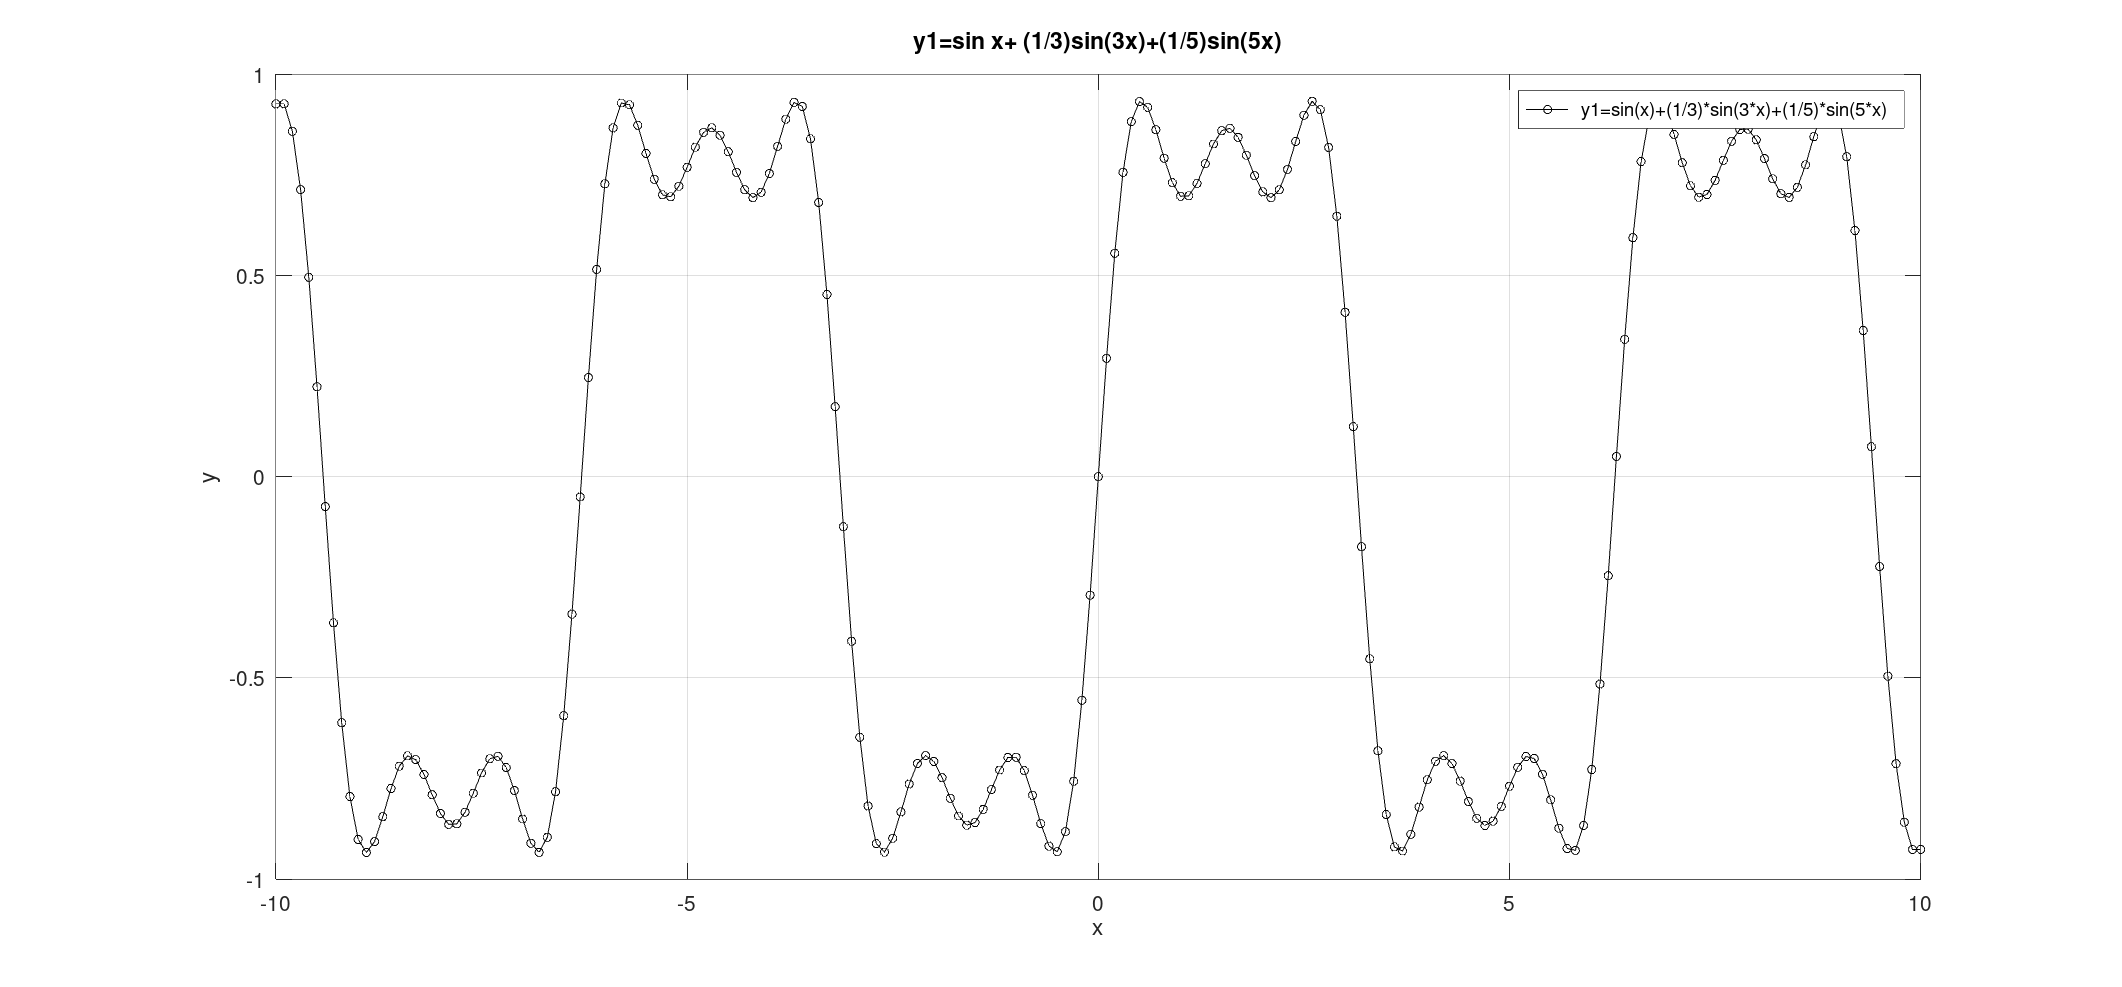
\includegraphics[width=\textwidth]{../octave/plot-sin.png}
    \captionof{figure}{\(y = \sin{x} + \frac{1}{3} \sin{3x} + \frac{1}{5} \sin{5x}\)}
\end{frame}

\begin{frame}
\frametitle{Построение графиков в Octave}
    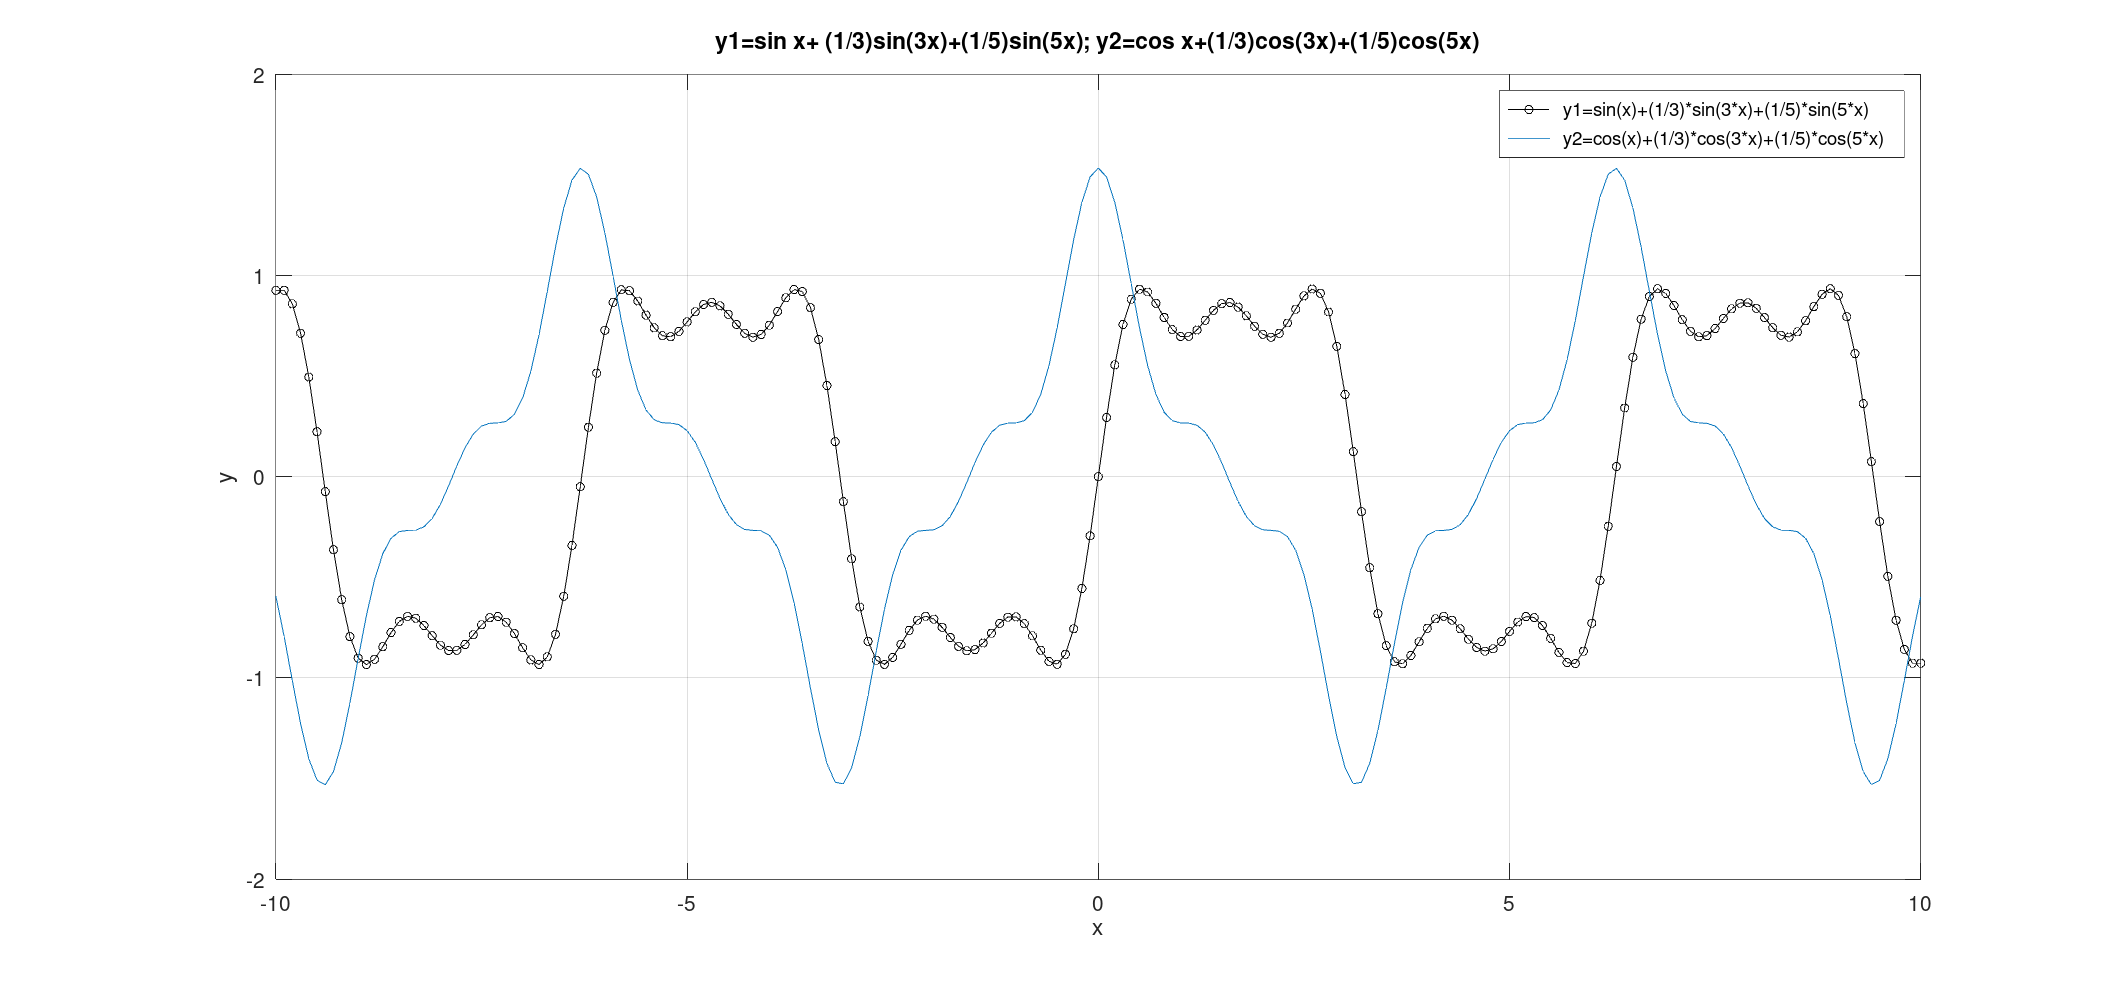
\includegraphics[width=\textwidth]{../octave/plot-sincos.png}
    \captionof{figure}{\(y1 = \sin{x} + \frac{1}{3} \sin{3x} + \frac{1}{5} \sin{5x},y2 = \cos{x} + \frac{1}{3} \cos`{3x} + \frac{1}{5} \cos{5x}\)}
\end{frame}

\begin{frame}
\frametitle{Разложение импульсного сигнала в частичный ряд Фурье}
    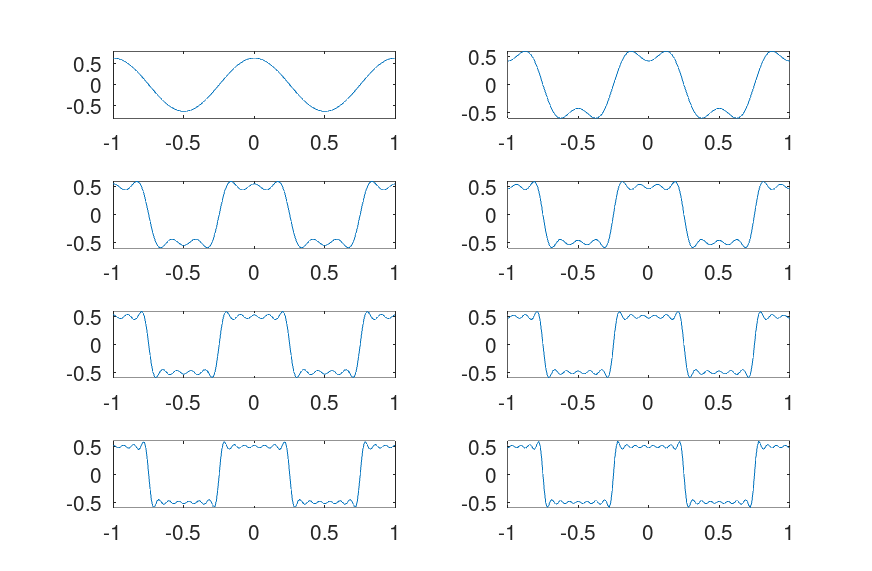
\includegraphics[width=\textwidth]{../octave/plot-meandr-cos.png}
    \captionof{figure}{графики меандра, с различным числом гармоник (косинусы).}
\end{frame}

\begin{frame}
\frametitle{Разложение импульсного сигнала в частичный ряд Фурье}
    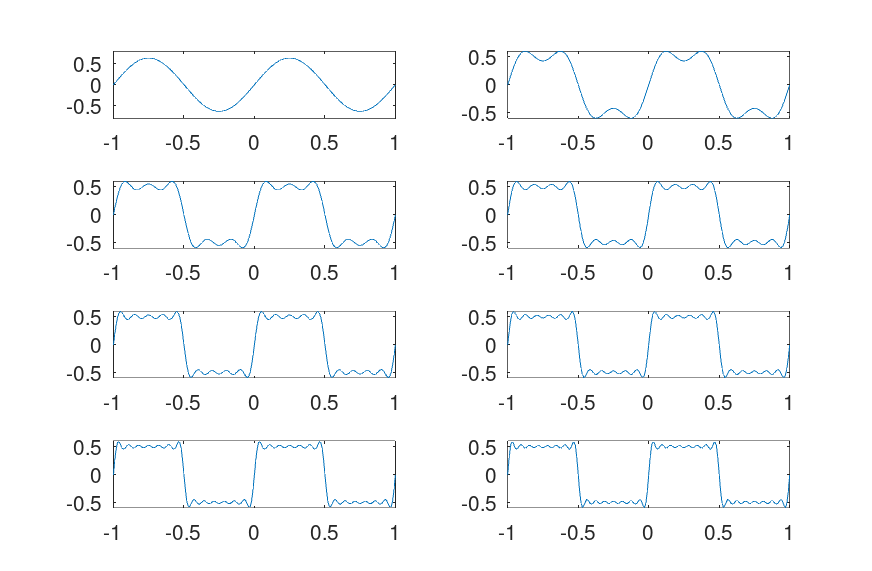
\includegraphics[width=\textwidth]{../octave/plot-meandr-sin.png}
    \captionof{figure}{Графики меандра, с различным числом гармоник (синусы).}
\end{frame}

\begin{frame}
\frametitle{Определение спектра и параметров сигнала}
            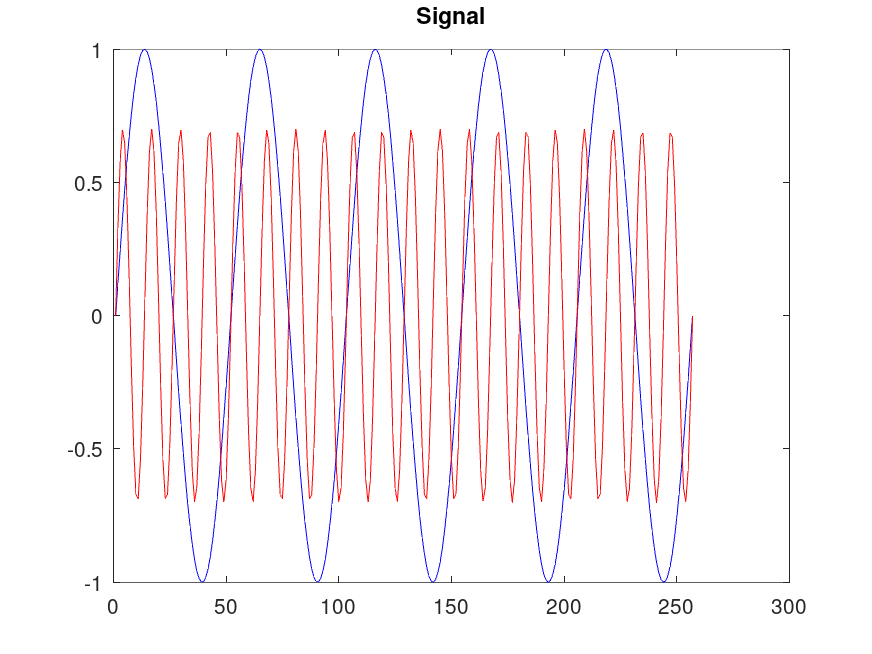
\includegraphics[width=\textwidth]{../octave/spectre1/signal/spectre.png}
            \captionof{figure}{Два синусоидальных сигнала разной частоты.}
\end{frame}

\begin{frame}
\frametitle{Определение спектра и параметров сигнала}
\begin{columns}
    \column{0.5\textwidth}
            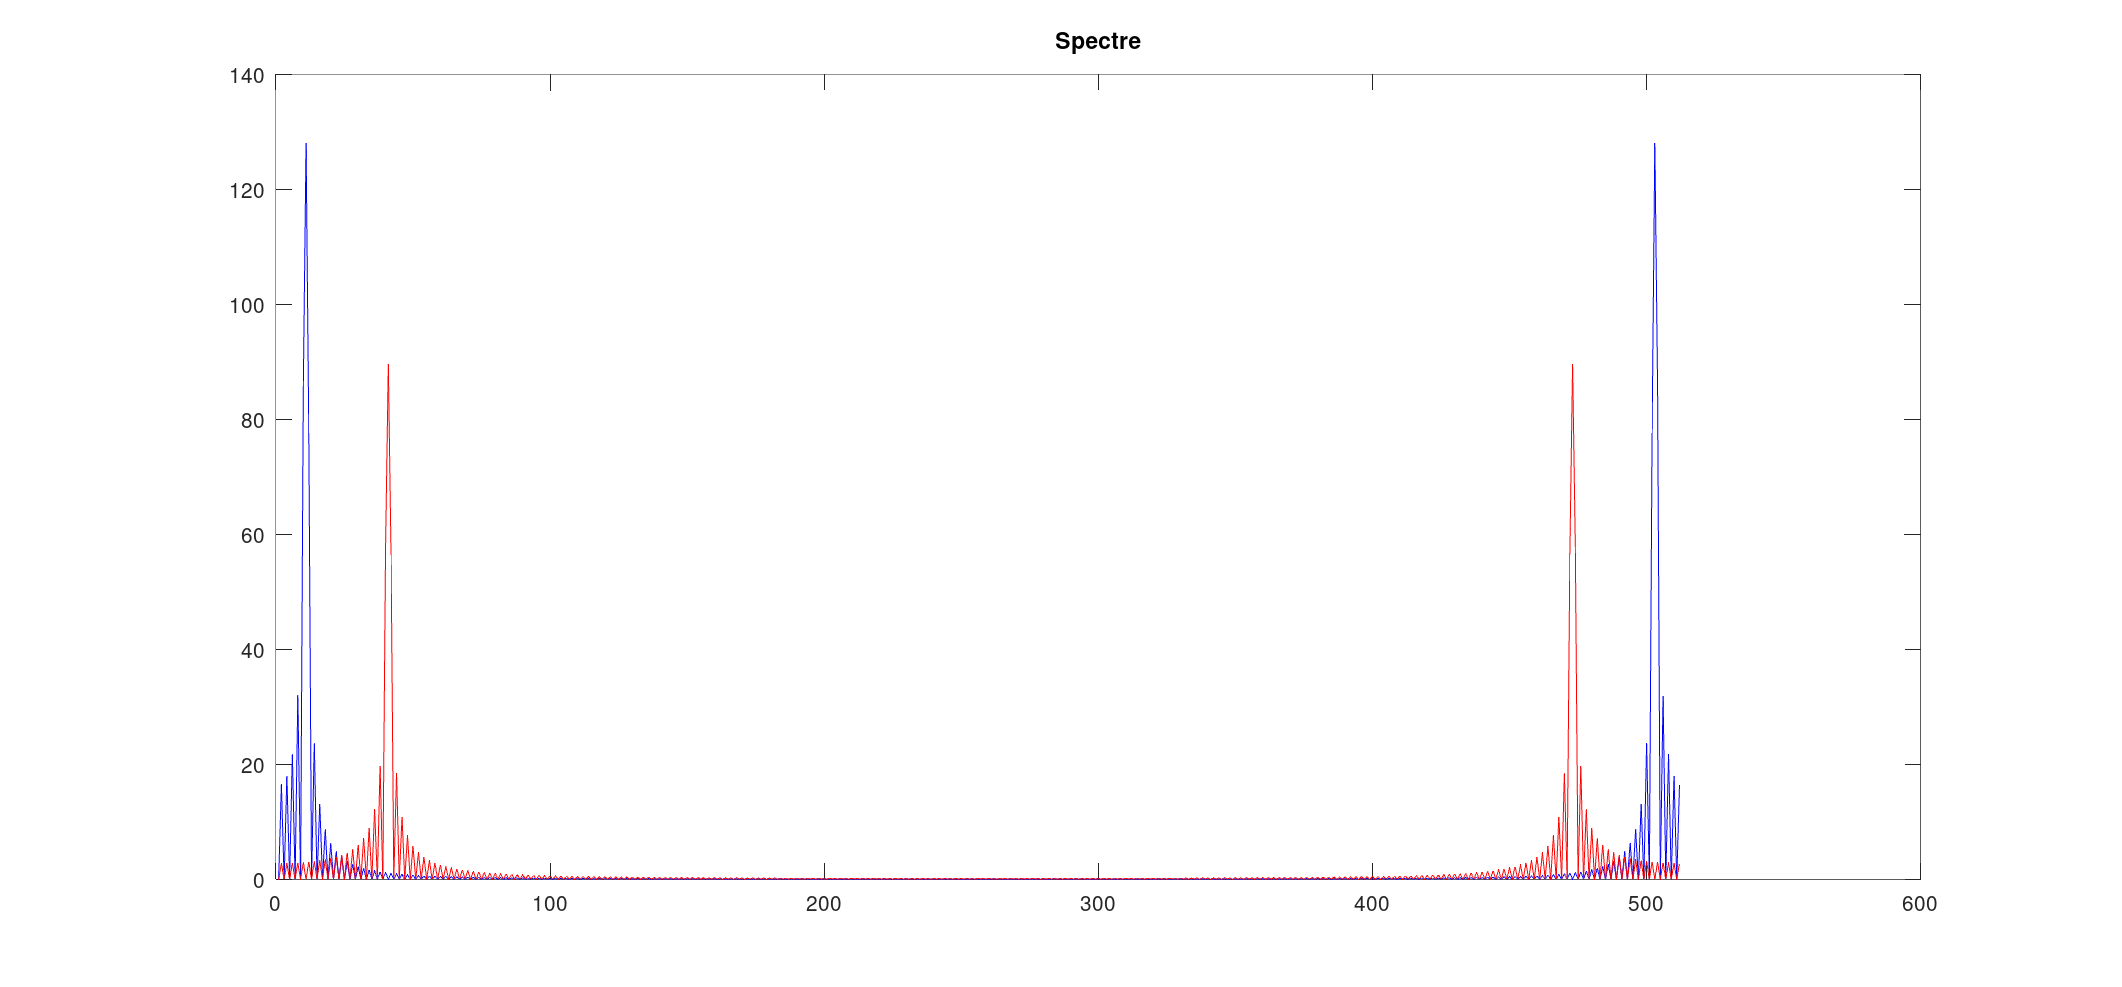
\includegraphics[width=\textwidth]{../octave/spectre1/spectre/spectre.png}
            \captionof{figure}{График спектров синусоидальных сигналов.}
    \column{0.5\textwidth}
            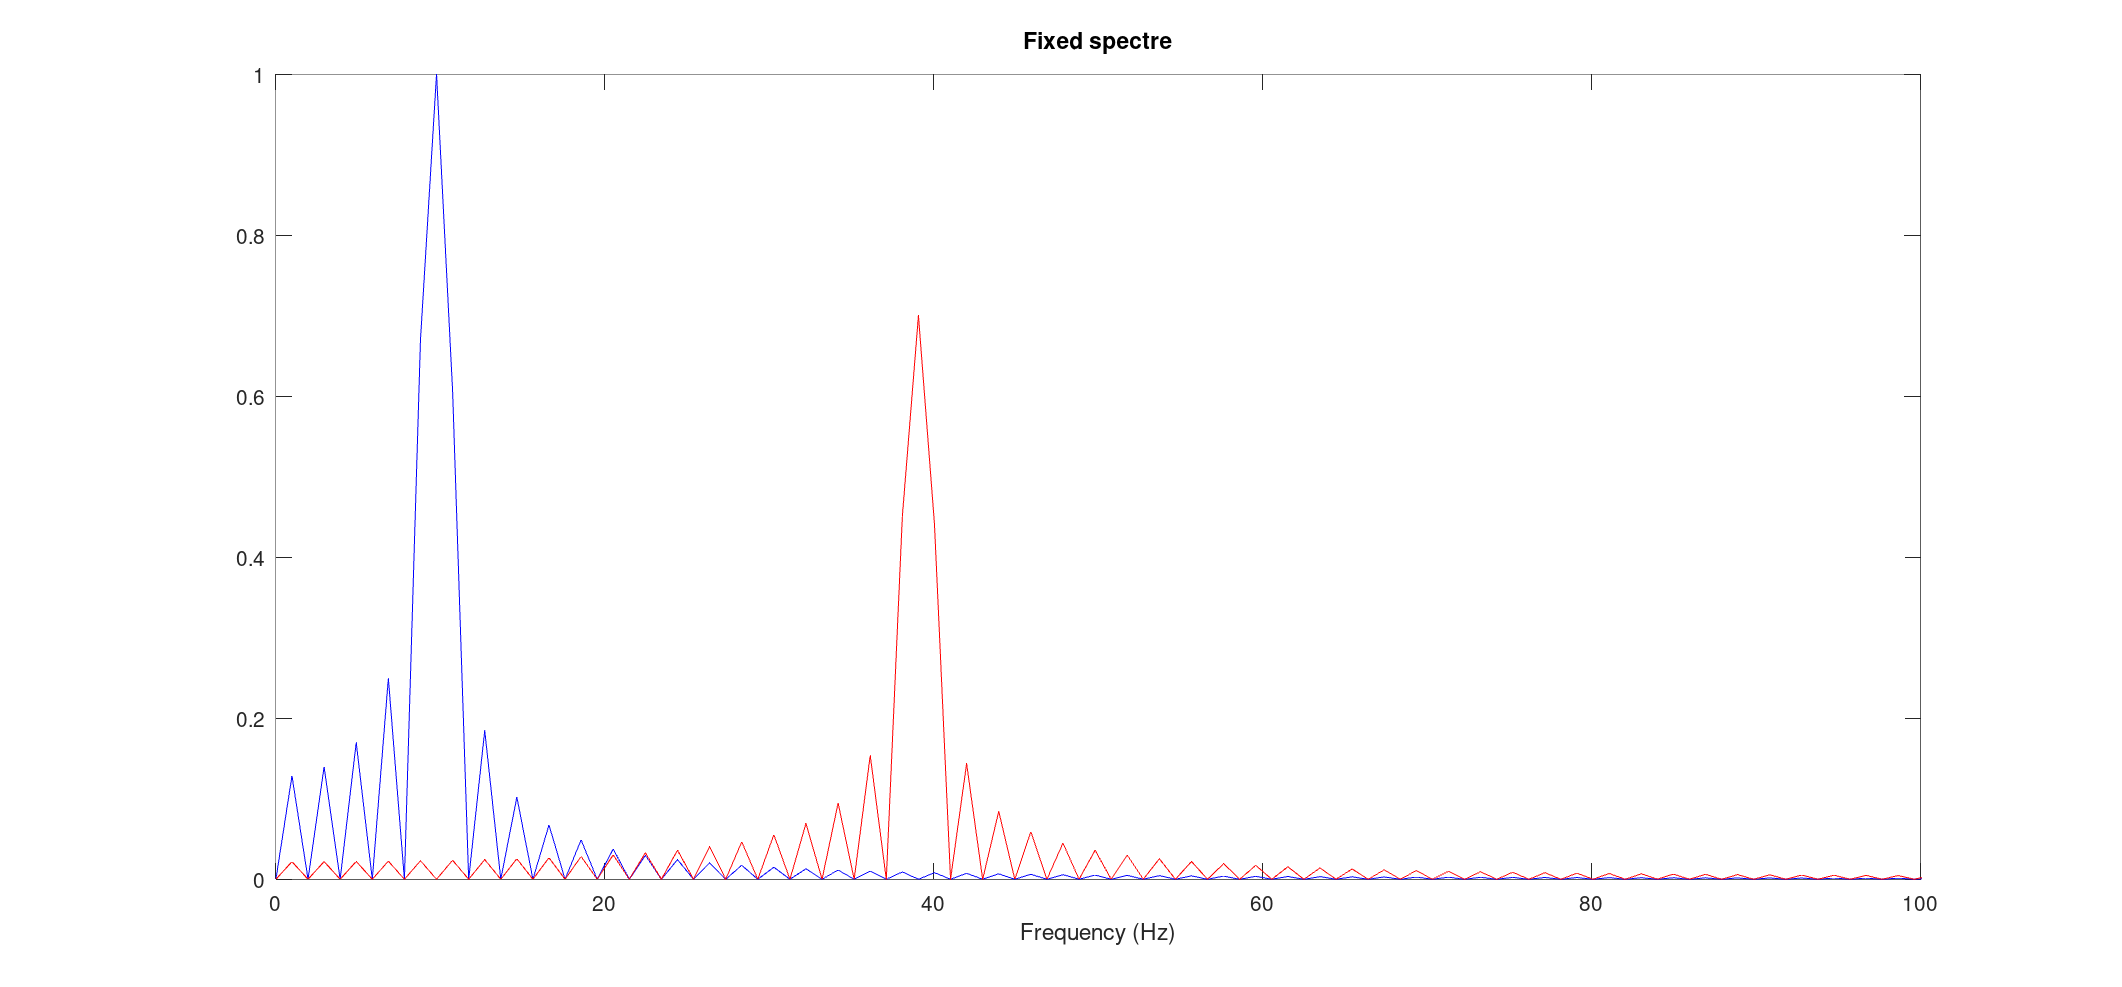
\includegraphics[width=\textwidth]{../octave/spectre1/spectre/spectre_fix.png}
            \captionof{figure}{Исправленный график спектров синусоидальных сигналов.}
\end{columns}
\end{frame}

\begin{frame}
\frametitle{Амплитудная модуляция}
            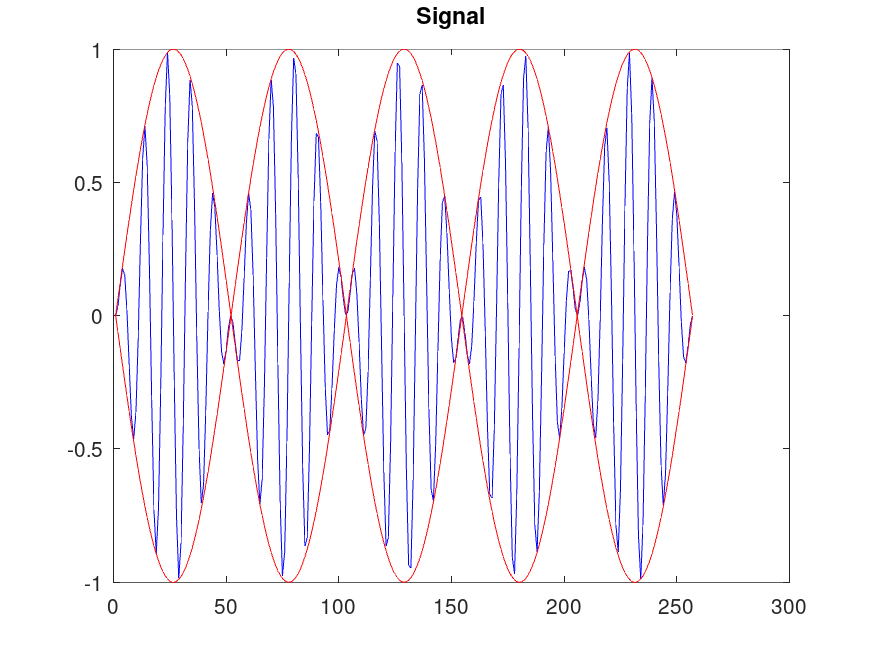
\includegraphics[width=\textwidth]{../octave/modulation/signal/am.png}
            \captionof{figure}{Сигнал и огибающая при амплитудной модуляции.}
\end{frame}

\begin{frame}
\frametitle{Амплитудная модуляция}
            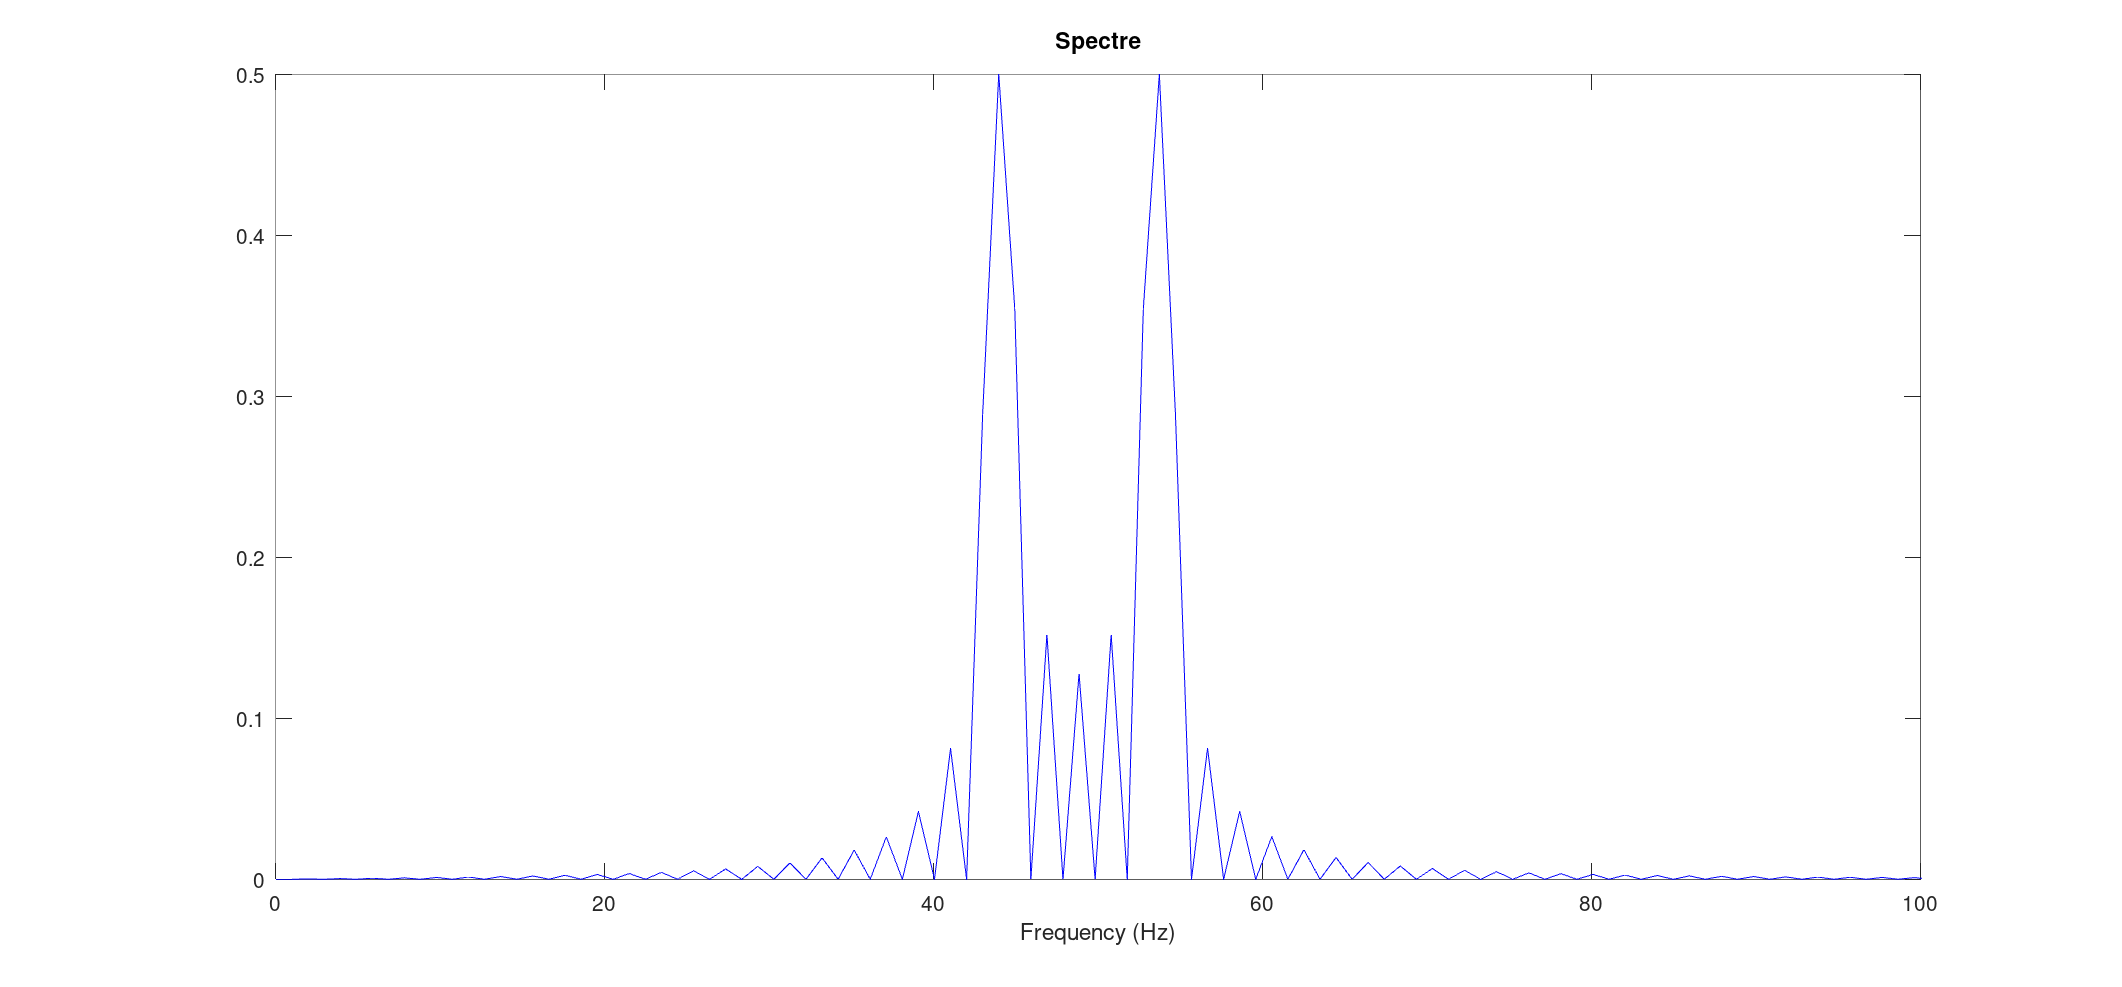
\includegraphics[width=\textwidth]{../octave/modulation/spectre/am.png}
            \captionof{figure}{Спектр сигнала при амплитудной модуляции.}
\end{frame}

\begin{frame}
\frametitle{Кодирование сигнала. Исследование свойства самосинхронизации сигнала}
\begin{columns}
    \column{0.5\textwidth}
            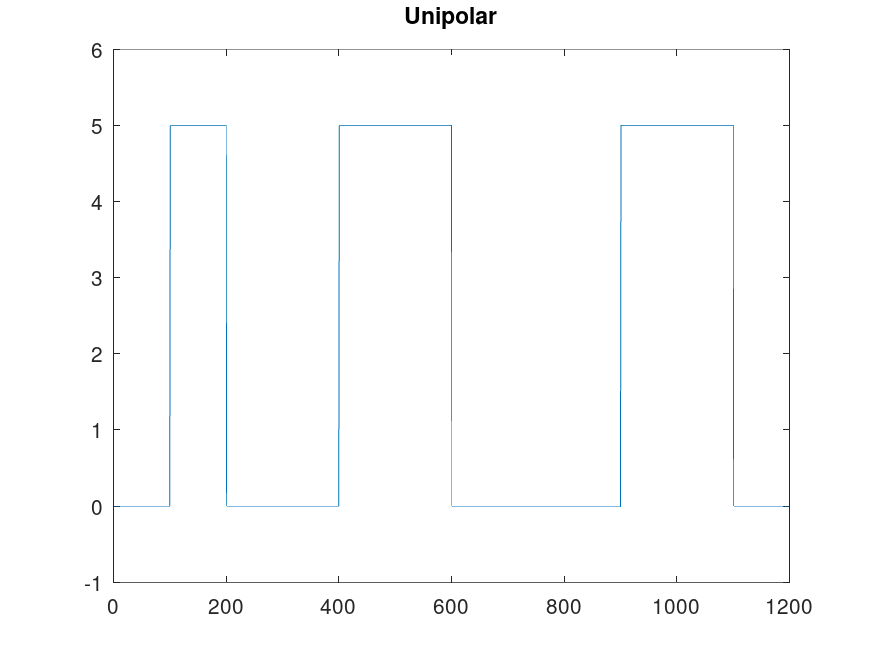
\includegraphics[width=\textwidth]{../octave/coding/signal/unipolar.png}
            \captionof{figure}{Униполярное кодирование.}
    \column{0.5\textwidth}
            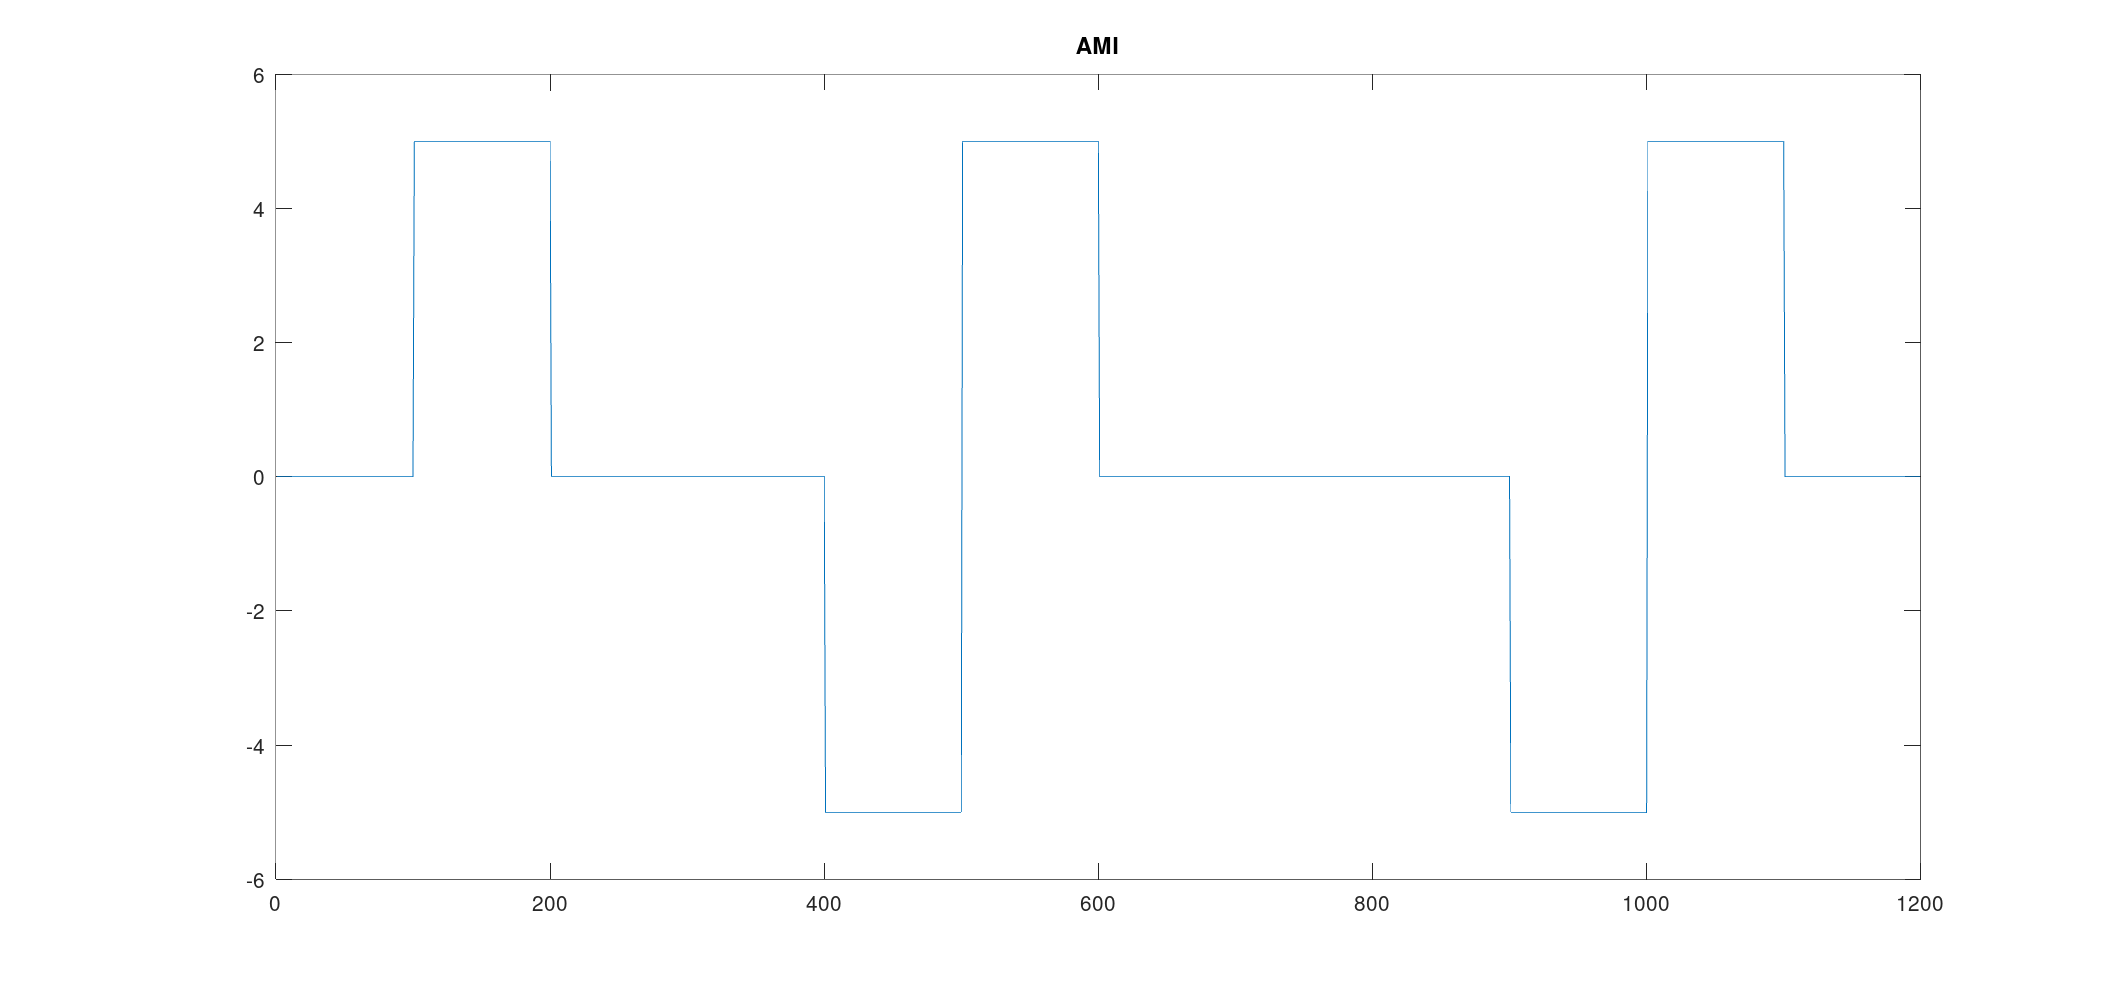
\includegraphics[width=\textwidth]{../octave/coding/signal/ami.png}
            \captionof{figure}{Кодирование AMI.}
\end{columns}
\end{frame}

\begin{frame}
\frametitle{Кодирование сигнала. Исследование свойства самосинхронизации сигнала}
\begin{columns}
    \column{0.5\textwidth}
            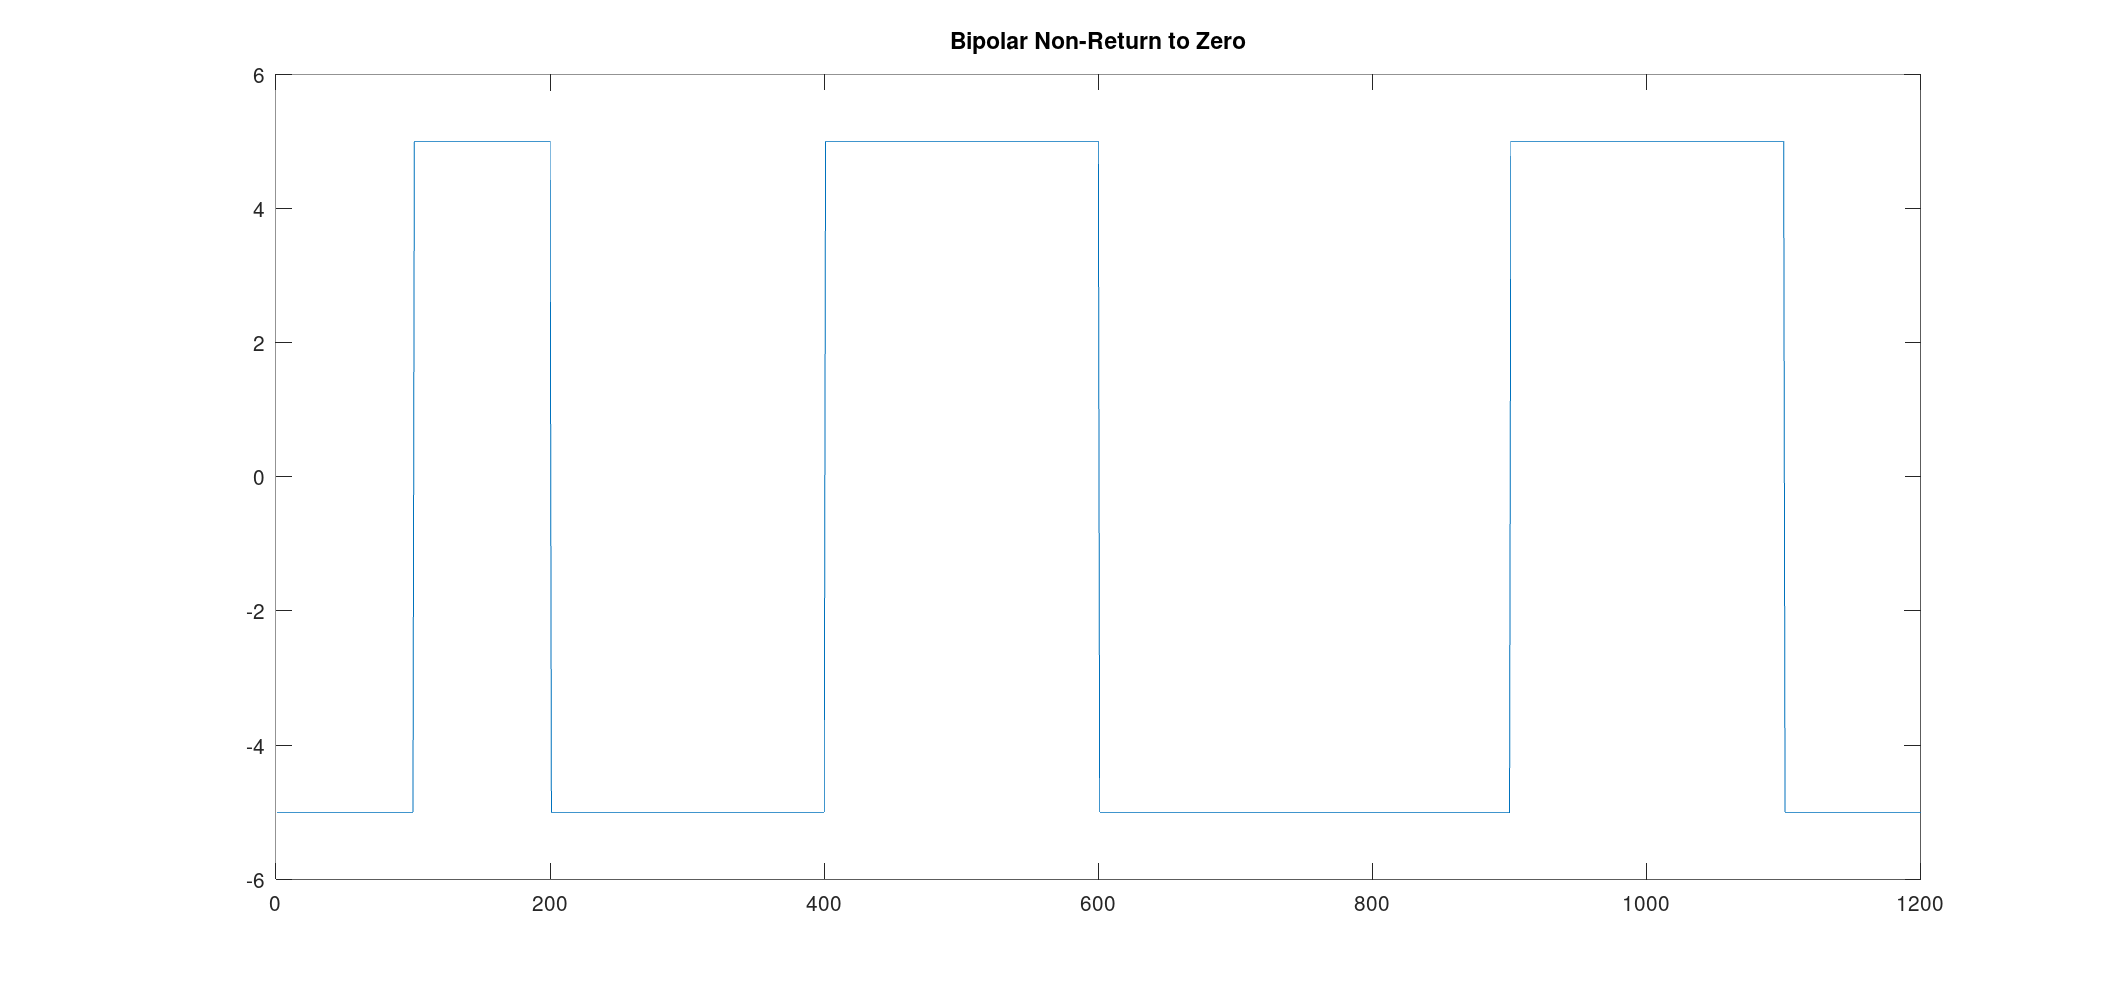
\includegraphics[width=\textwidth]{../octave/coding/signal/bipolarnrz.png}
            \captionof{figure}{Кодирование NRZ}
    \column{0.5\textwidth}
            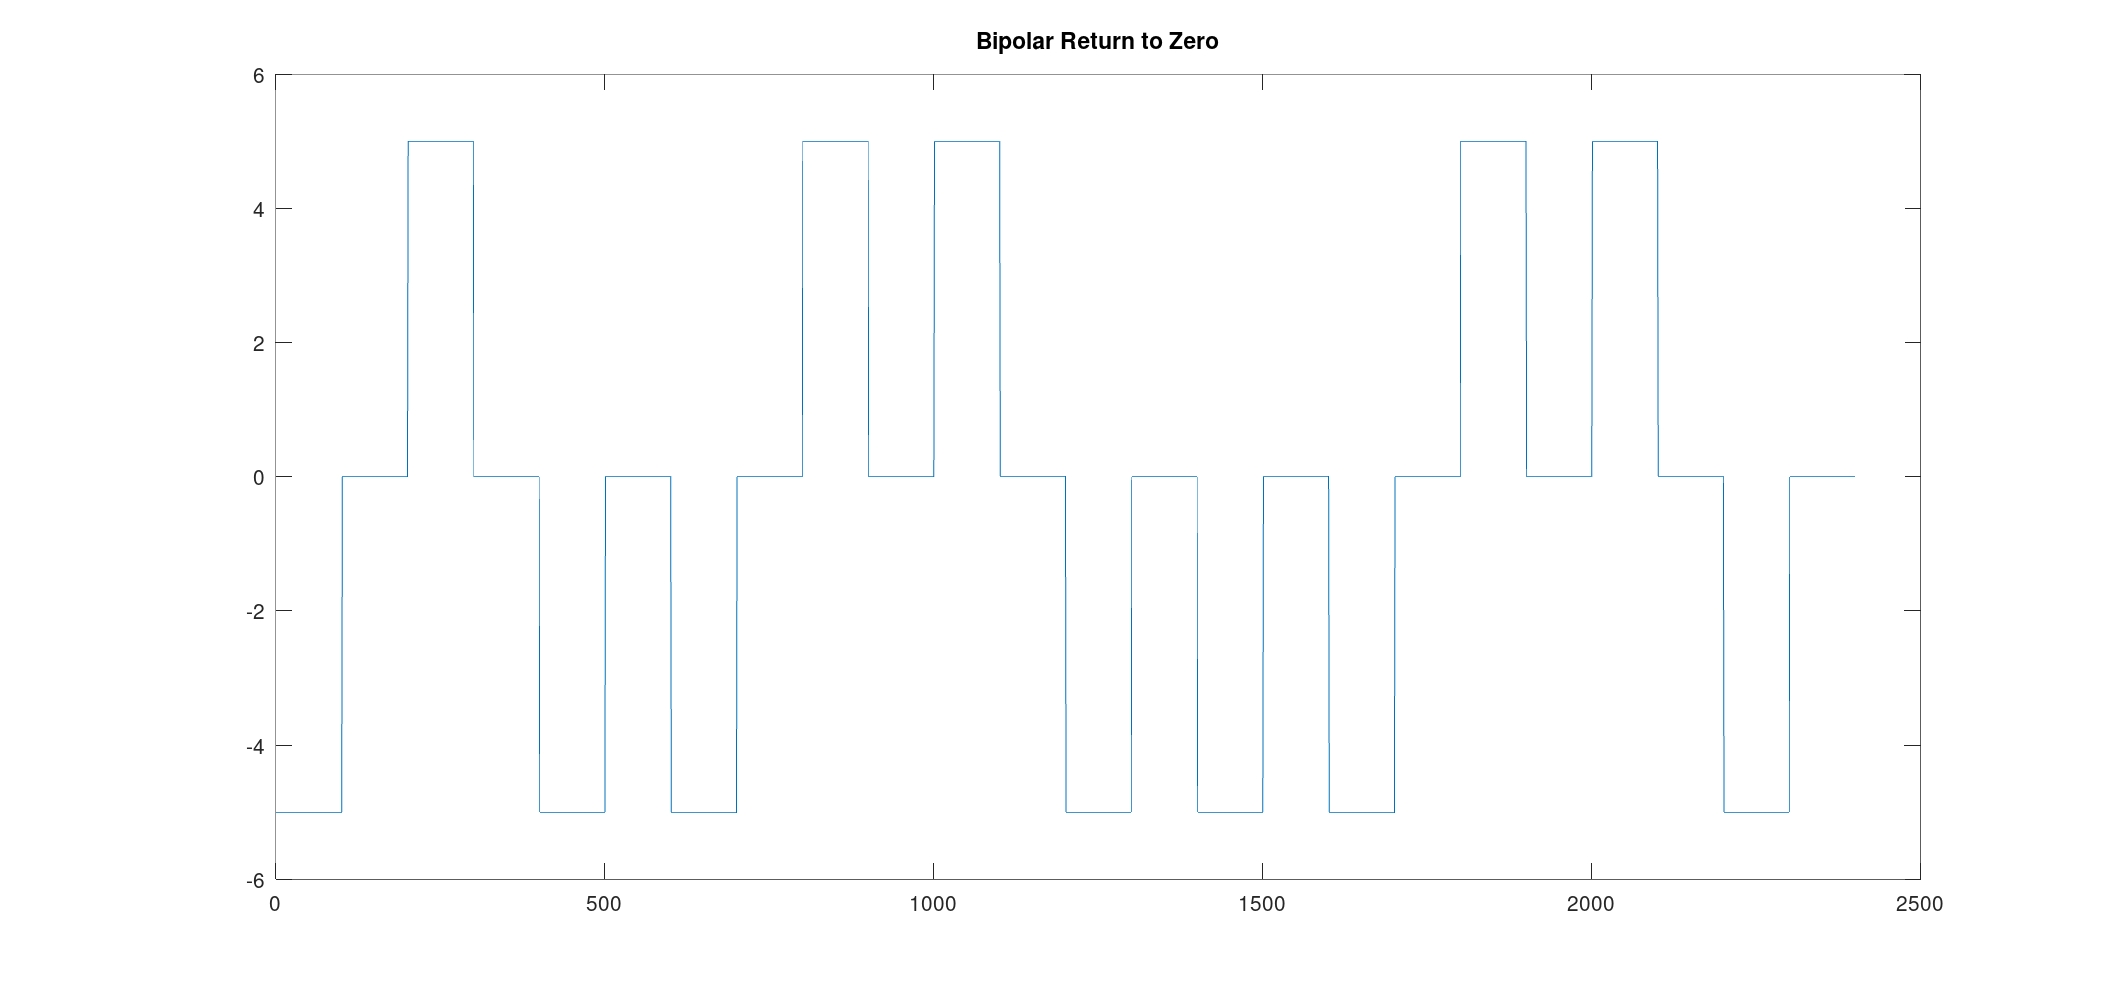
\includegraphics[width=\textwidth]{../octave/coding/signal/bipolarrz.png}
            \captionof{figure}{Кодирование RZ}
\end{columns}
\end{frame}

\begin{frame}
\frametitle{Кодирование сигнала. Исследование свойства самосинхронизации сигнала}
\begin{columns}
    \column{0.5\textwidth}
            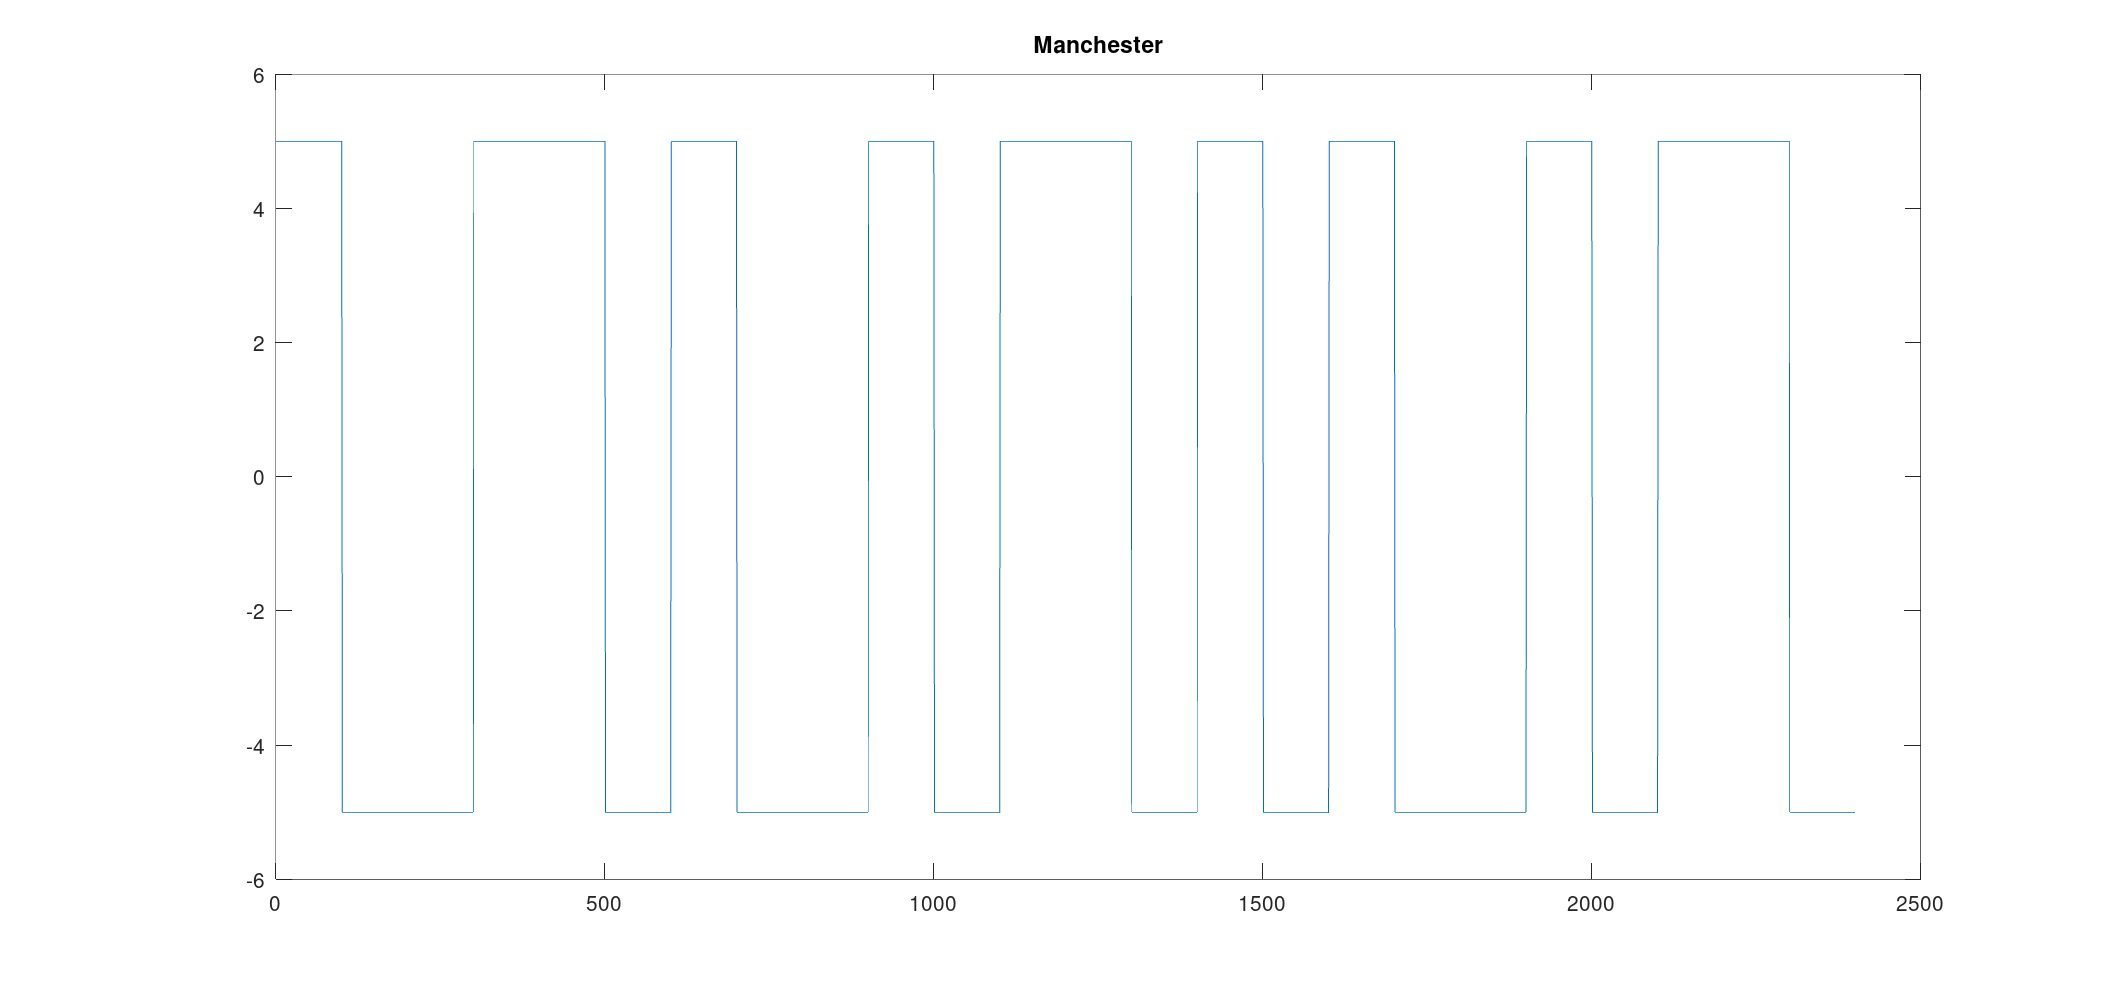
\includegraphics[width=\textwidth]{../octave/coding/signal/manchester.png}
            \captionof{figure}{Манчестрерское кодирование.}
    \column{0.5\textwidth}
            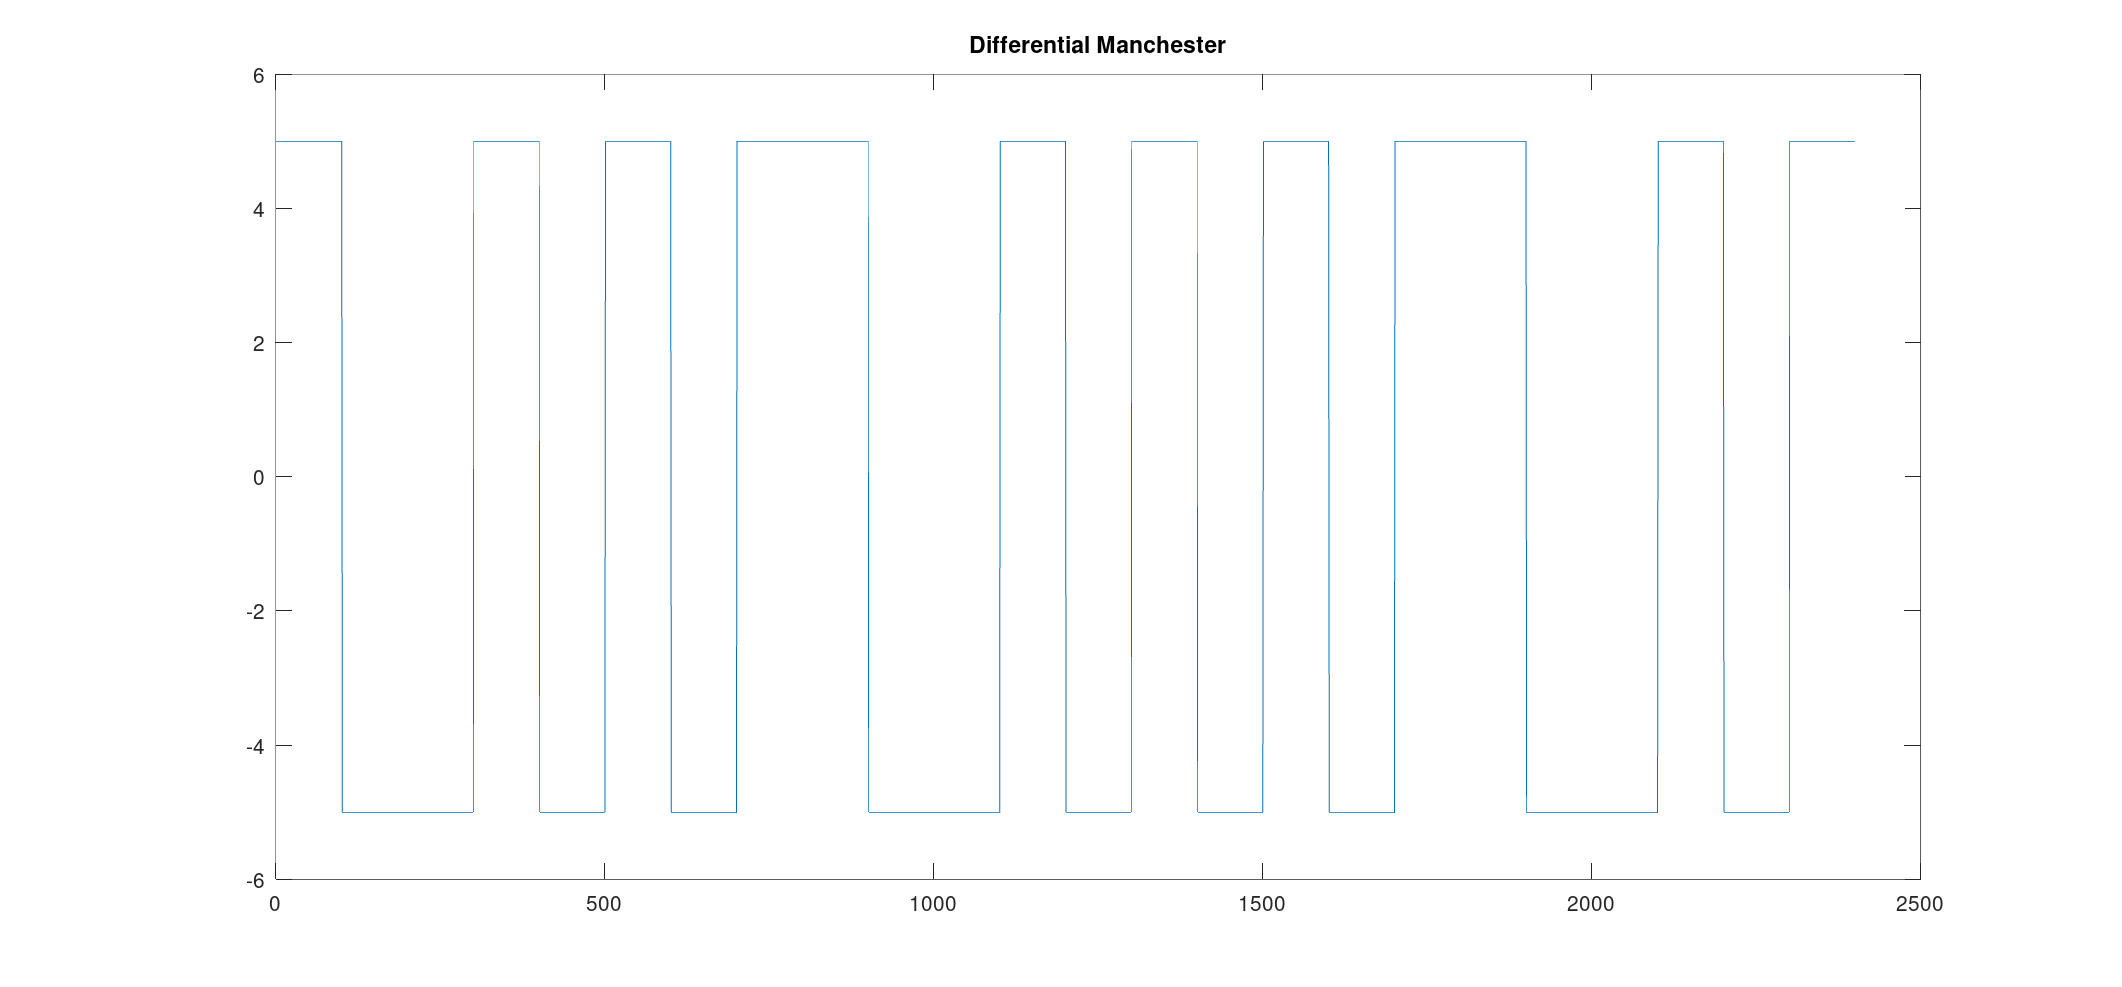
\includegraphics[width=\textwidth]{../octave/coding/signal/diffmanc.png}
            \captionof{figure}{Дифференциальное манчестерское кодирование.}
\end{columns}
\end{frame}


\begin{frame}
\frametitle{Кодирование сигнала. Исследование свойства самосинхронизации сигнала}
\begin{columns}
    \column{0.5\textwidth}
            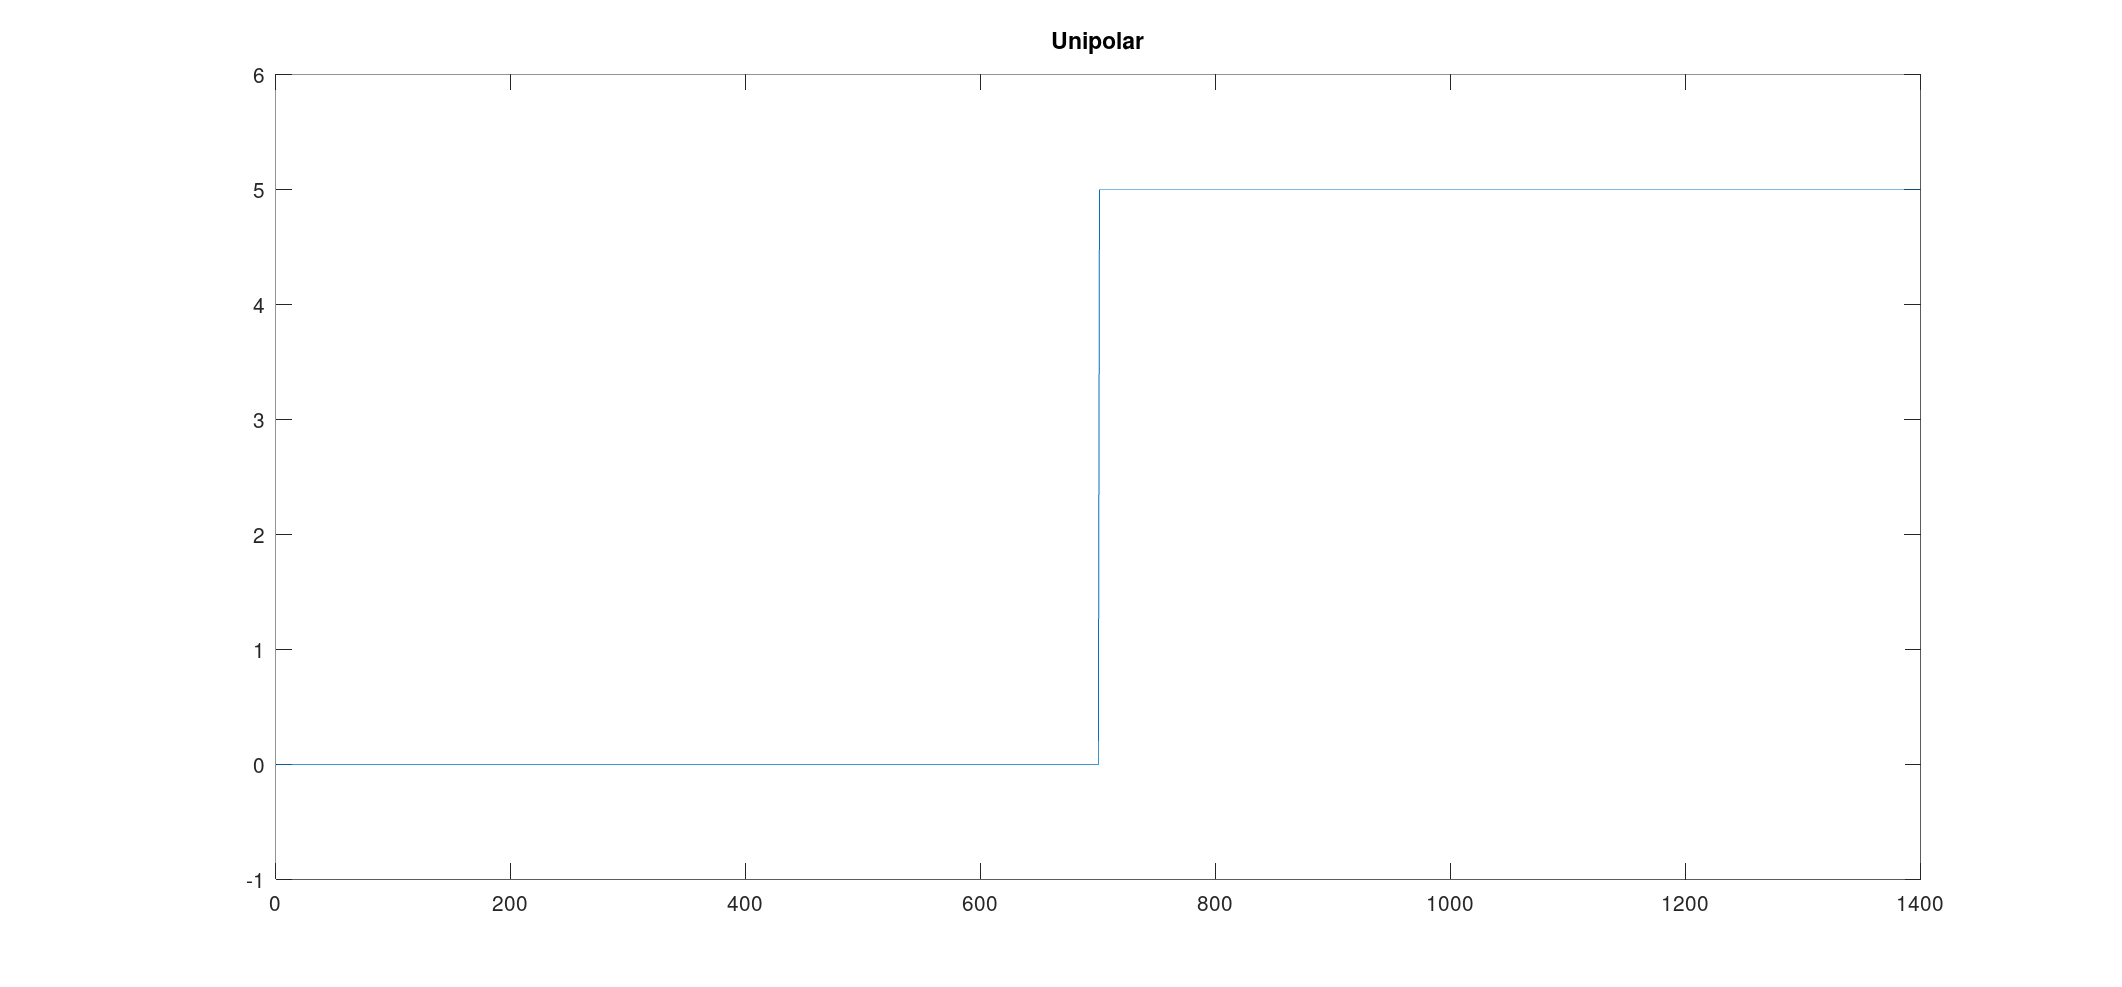
\includegraphics[width=\textwidth]{../octave/coding/sync/unipolar.png}
            \captionof{figure}{Униполярное кодирование: нет синхронизации.}
    \column{0.5\textwidth}
            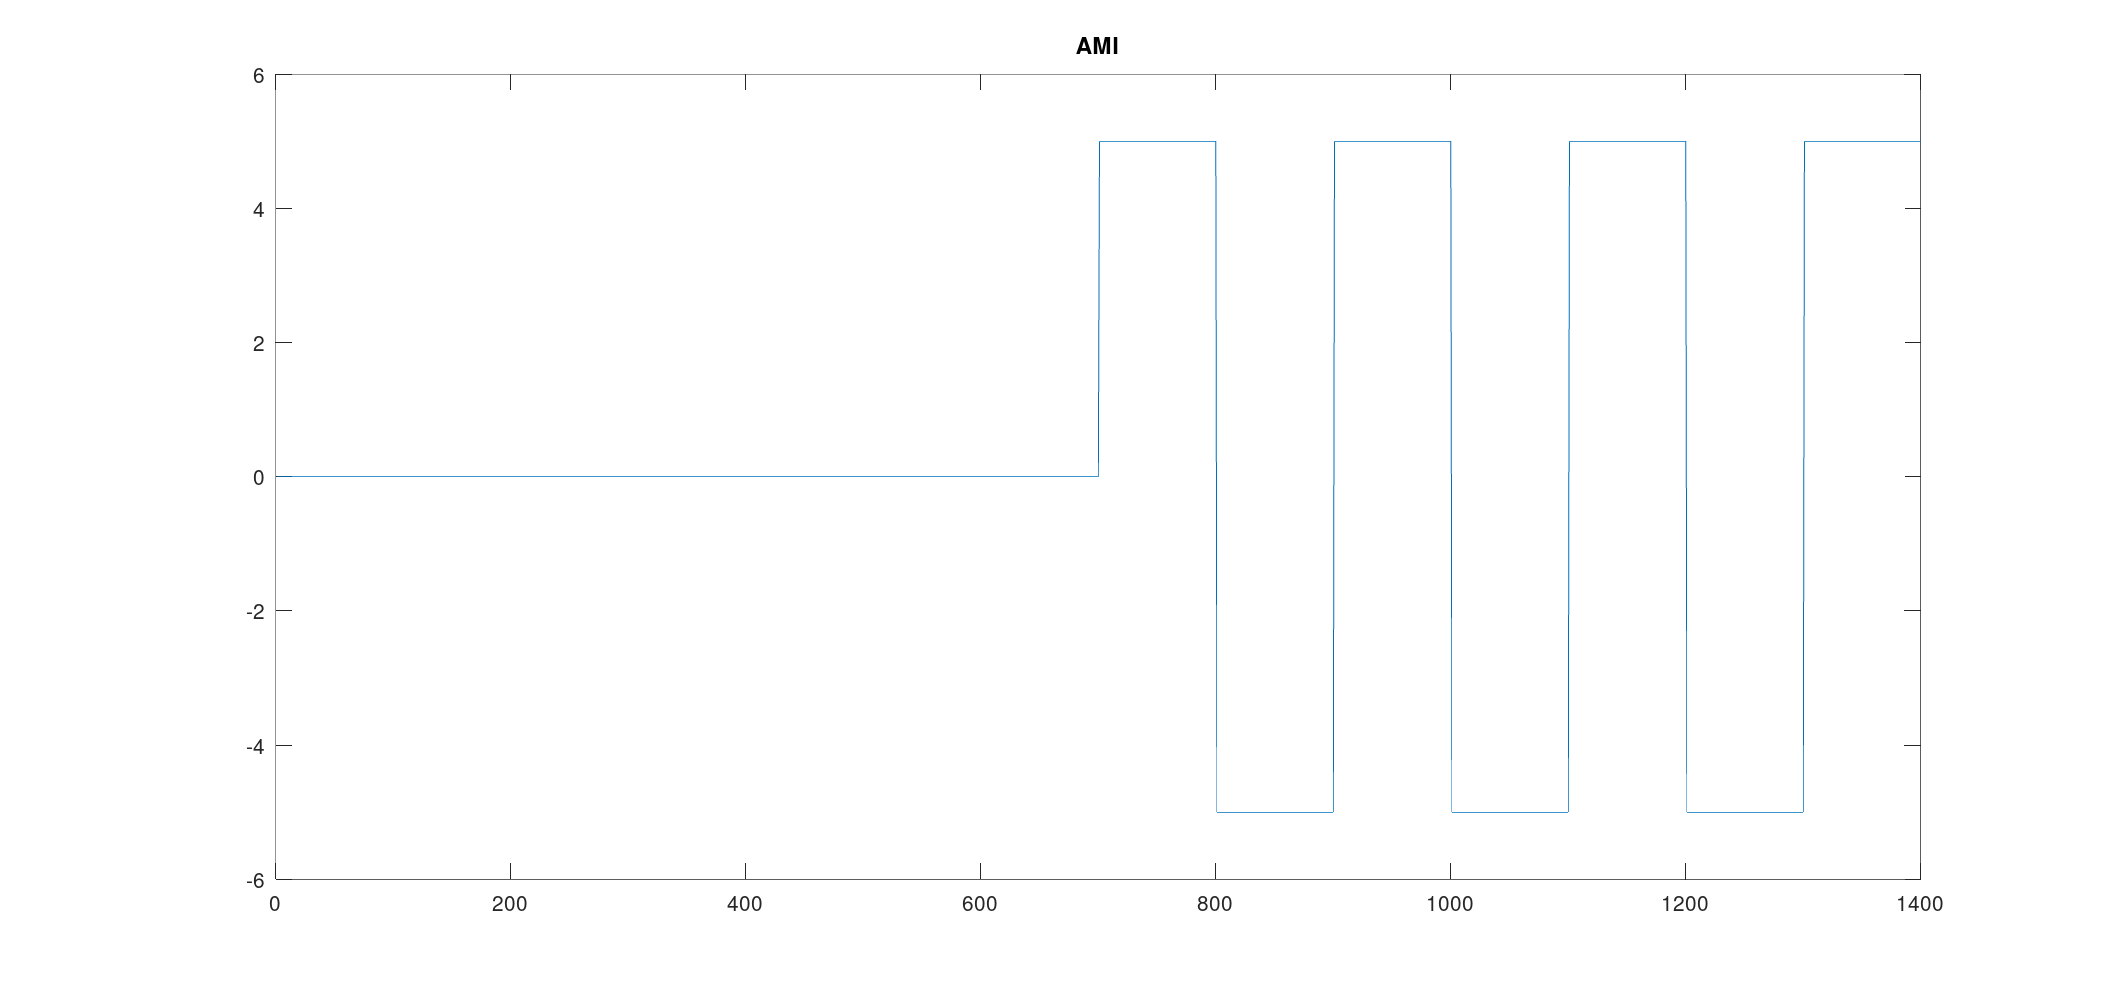
\includegraphics[width=\textwidth]{../octave/coding/sync/ami.png}
            \captionof{figure}{Кодирование AMI: самосинхронизация при наличии сигнала.}
\end{columns}
\end{frame}

\begin{frame}
\frametitle{Кодирование сигнала. Исследование свойства самосинхронизации сигнала}
\begin{columns}
    \column{0.5\textwidth}
            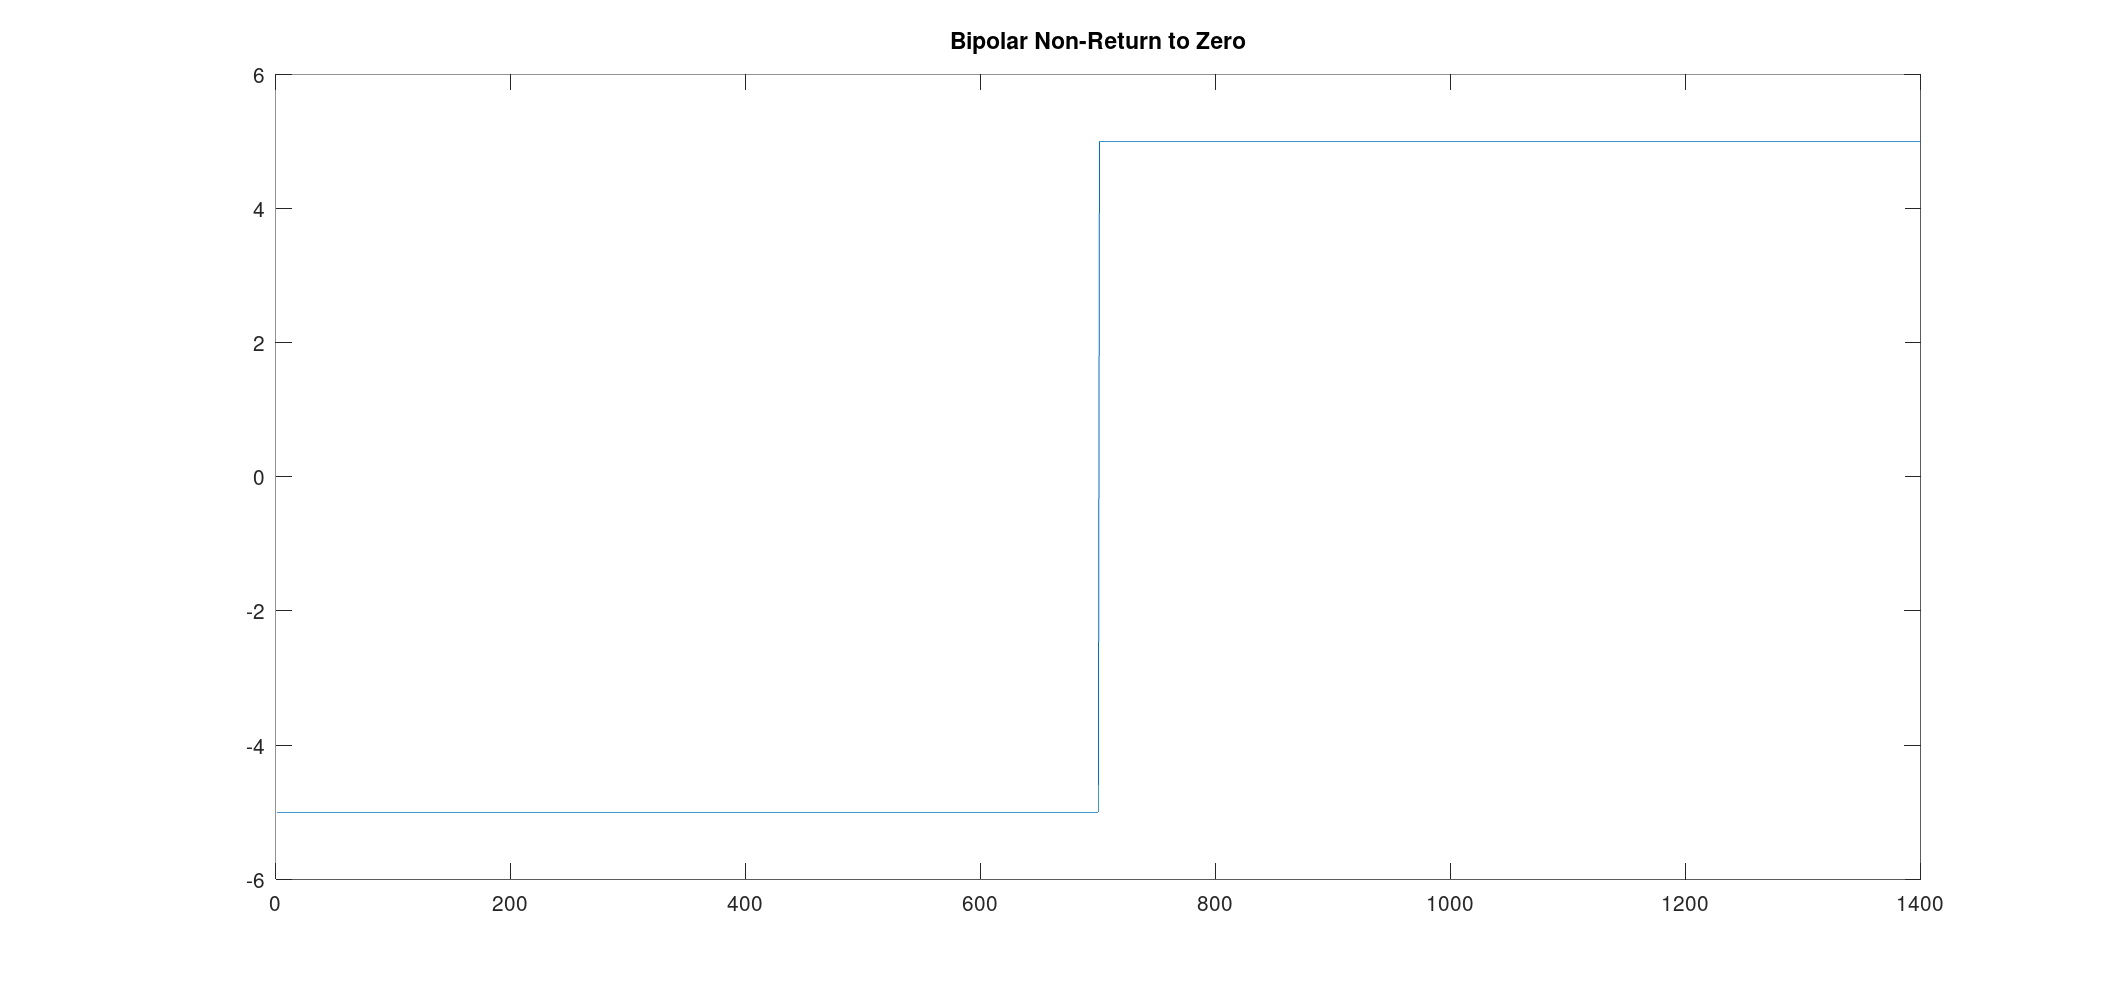
\includegraphics[width=\textwidth]{../octave/coding/sync/bipolarnrz.png}
            \captionof{figure}{Кодирование NRZ: нет самосинхронизации.}
    \column{0.5\textwidth}
            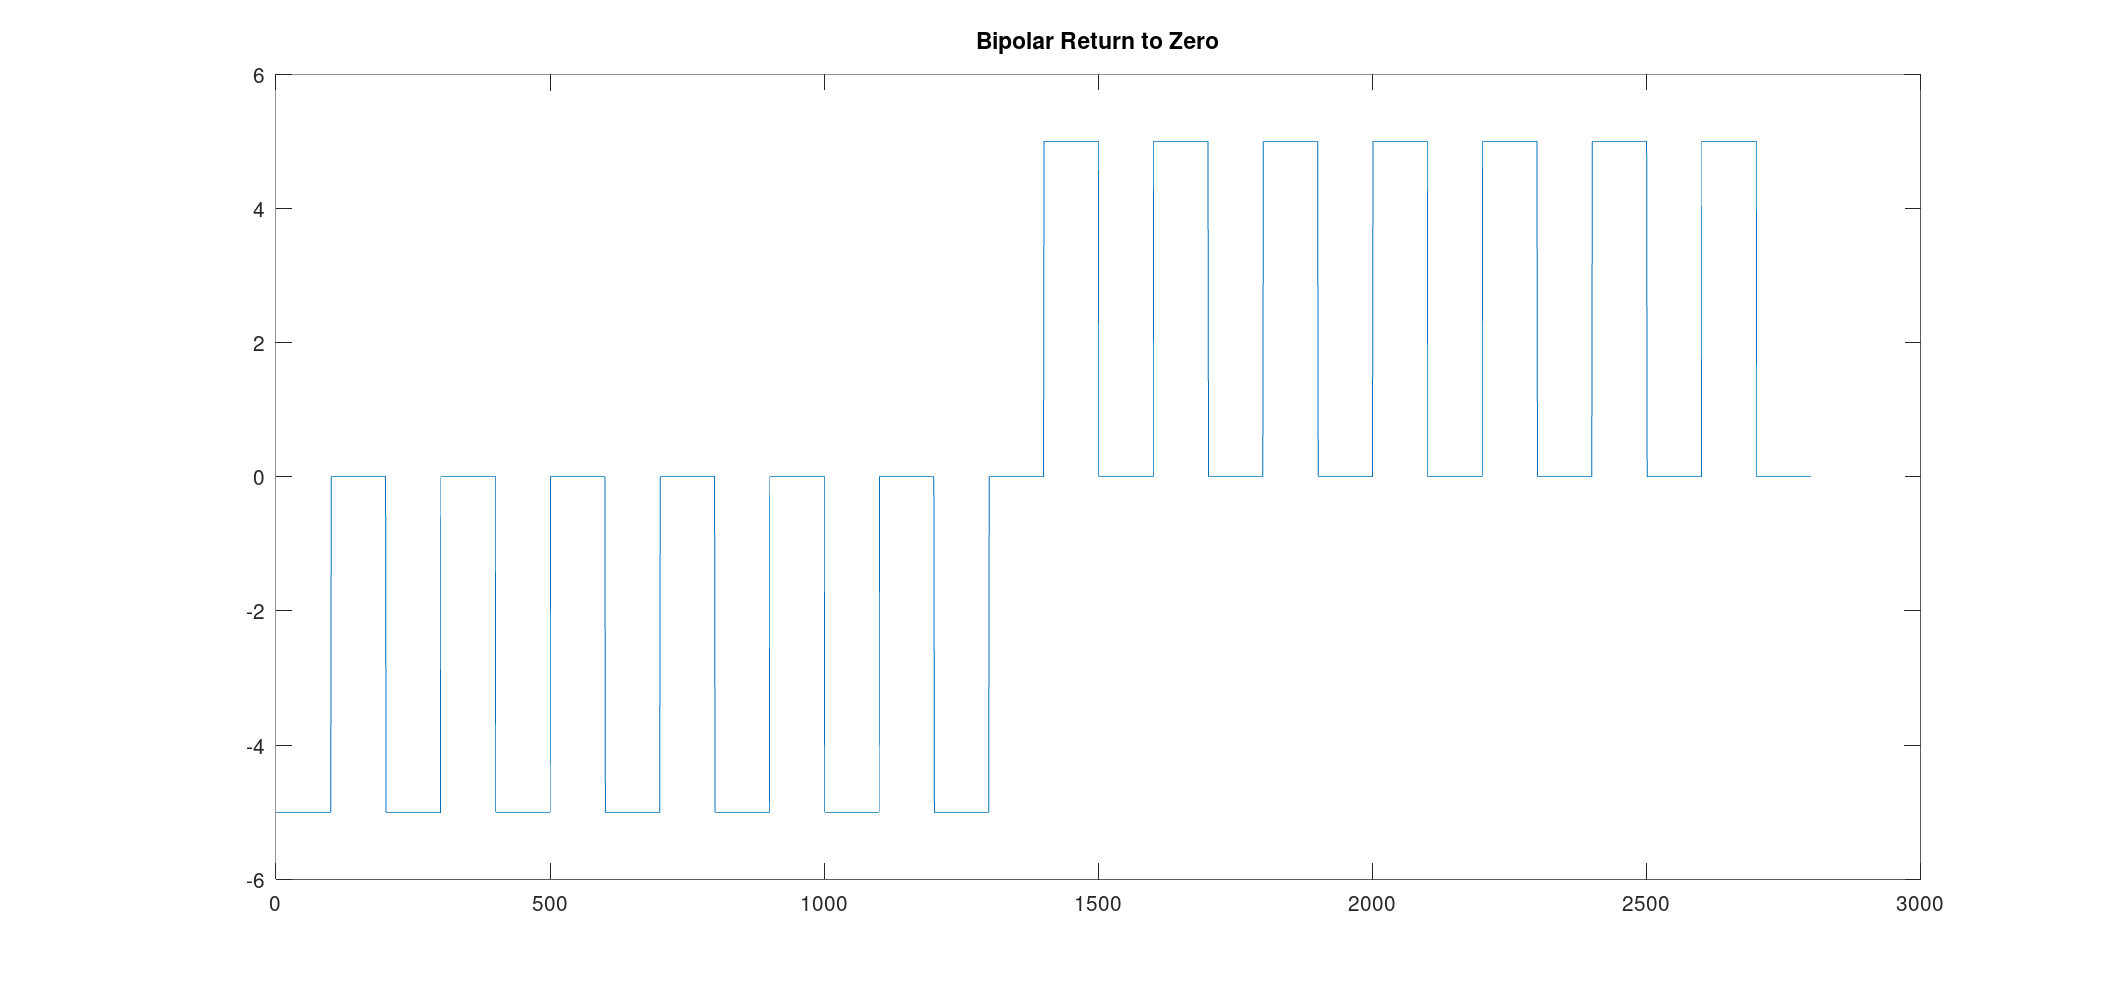
\includegraphics[width=\textwidth]{../octave/coding/sync/bipolarrz.png}
            \captionof{figure}{Кодирование RZ: есть самосинхронизация}
\end{columns}
\end{frame}

\begin{frame}
\frametitle{Кодирование сигнала. Исследование свойства самосинхронизации сигнала}
\begin{columns}
    \column{0.5\textwidth}
            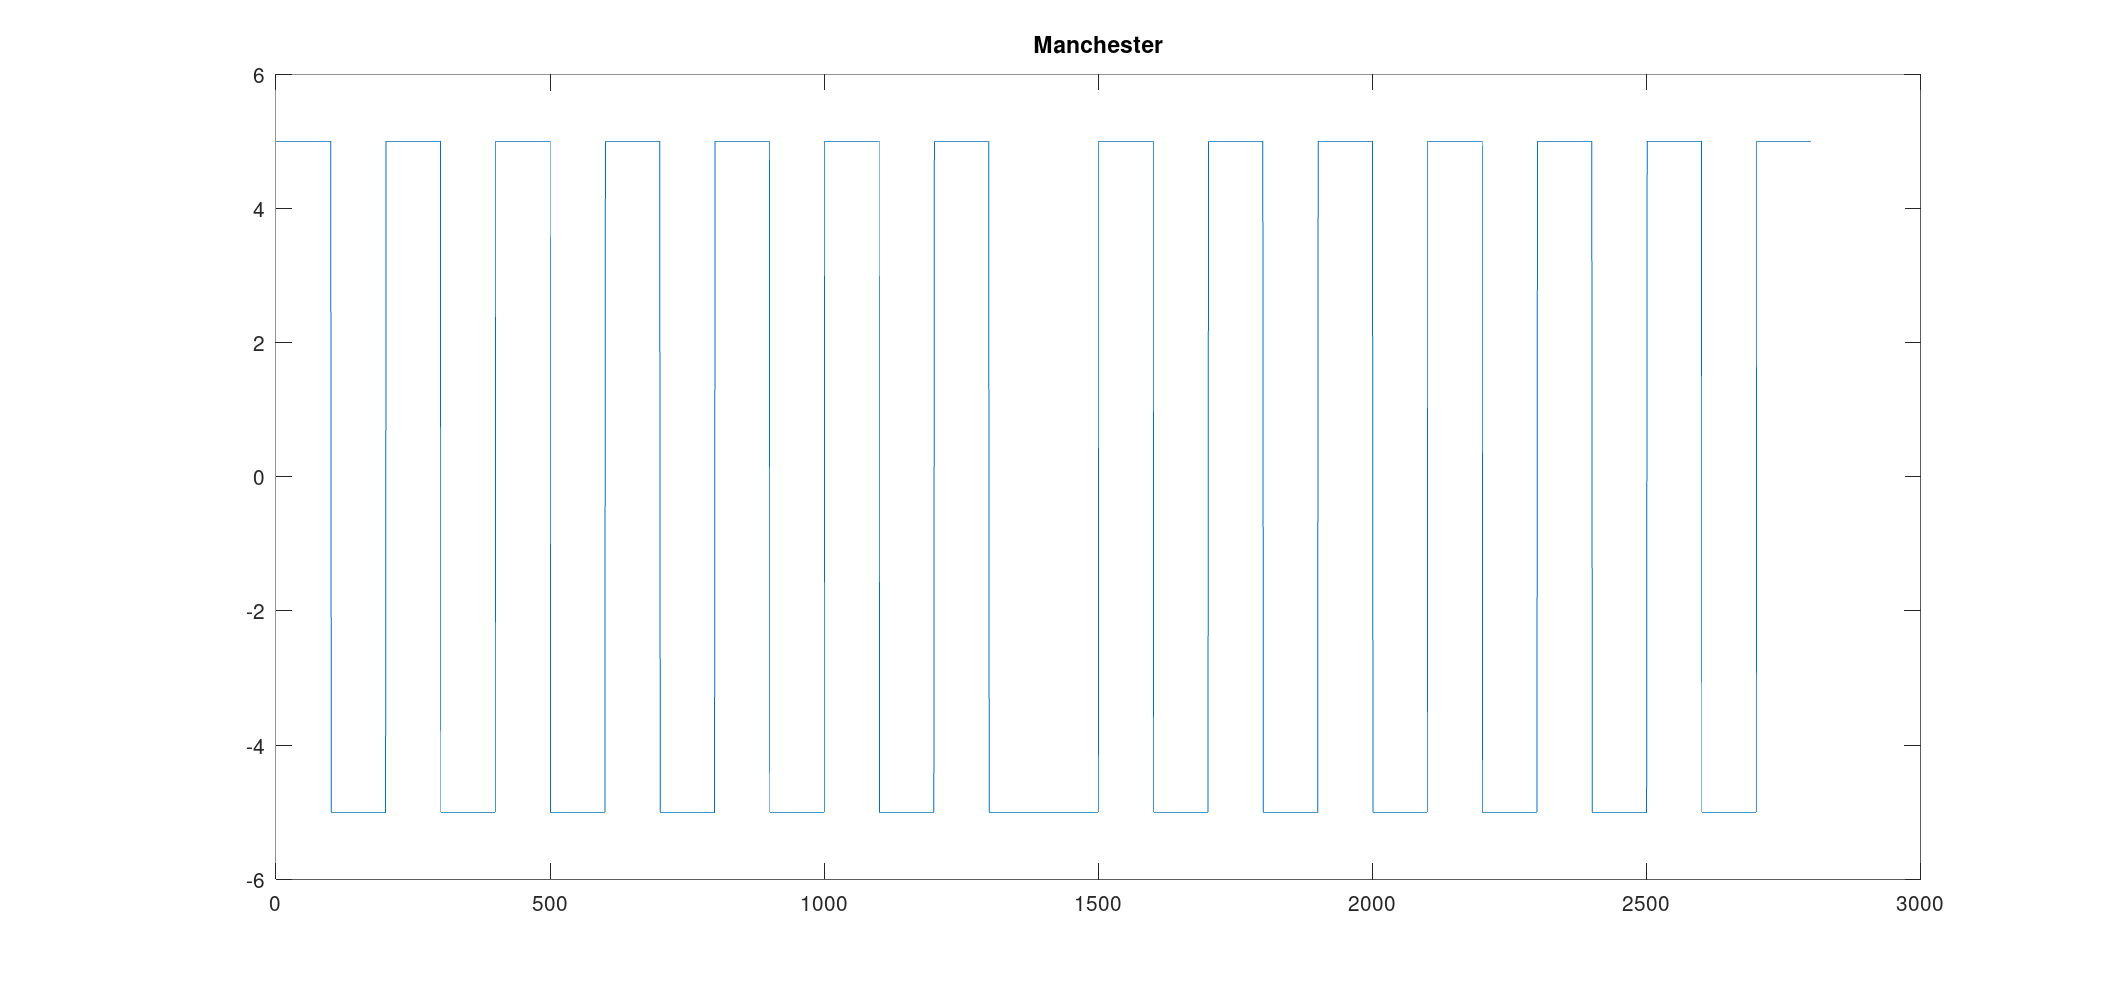
\includegraphics[width=\textwidth]{../octave/coding/sync/manchester.png}
            \captionof{figure}{Манчестрерское кодирование: есть самосинхронизация}
    \column{0.5\textwidth}
            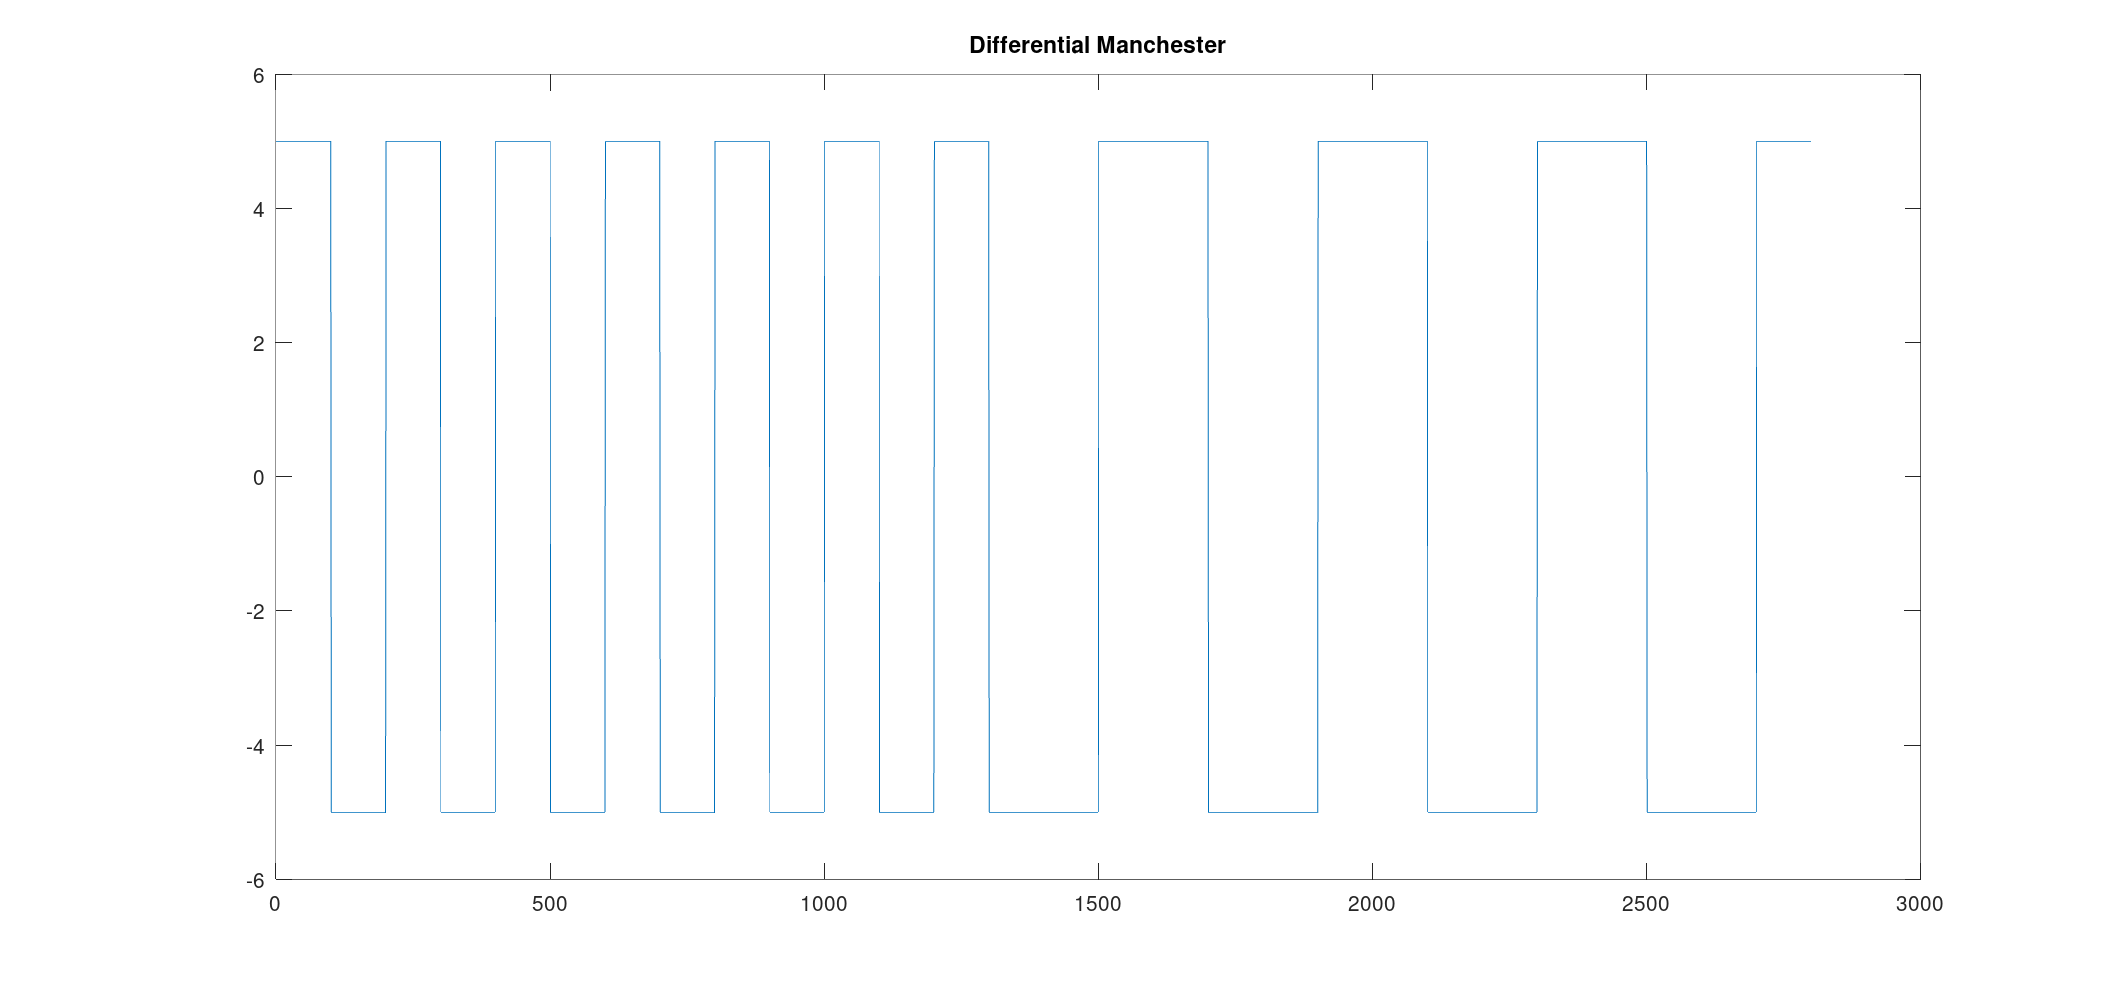
\includegraphics[width=\textwidth]{../octave/coding/sync/diffmanc.png}
            \captionof{figure}{Дифференциальное манчестерское кодирование: есть самосинхронизация}
\end{columns}
\end{frame}


\begin{frame}
\frametitle{Кодирование сигнала. Исследование свойства самосинхронизации сигнала}
\begin{columns}
    \column{0.5\textwidth}
            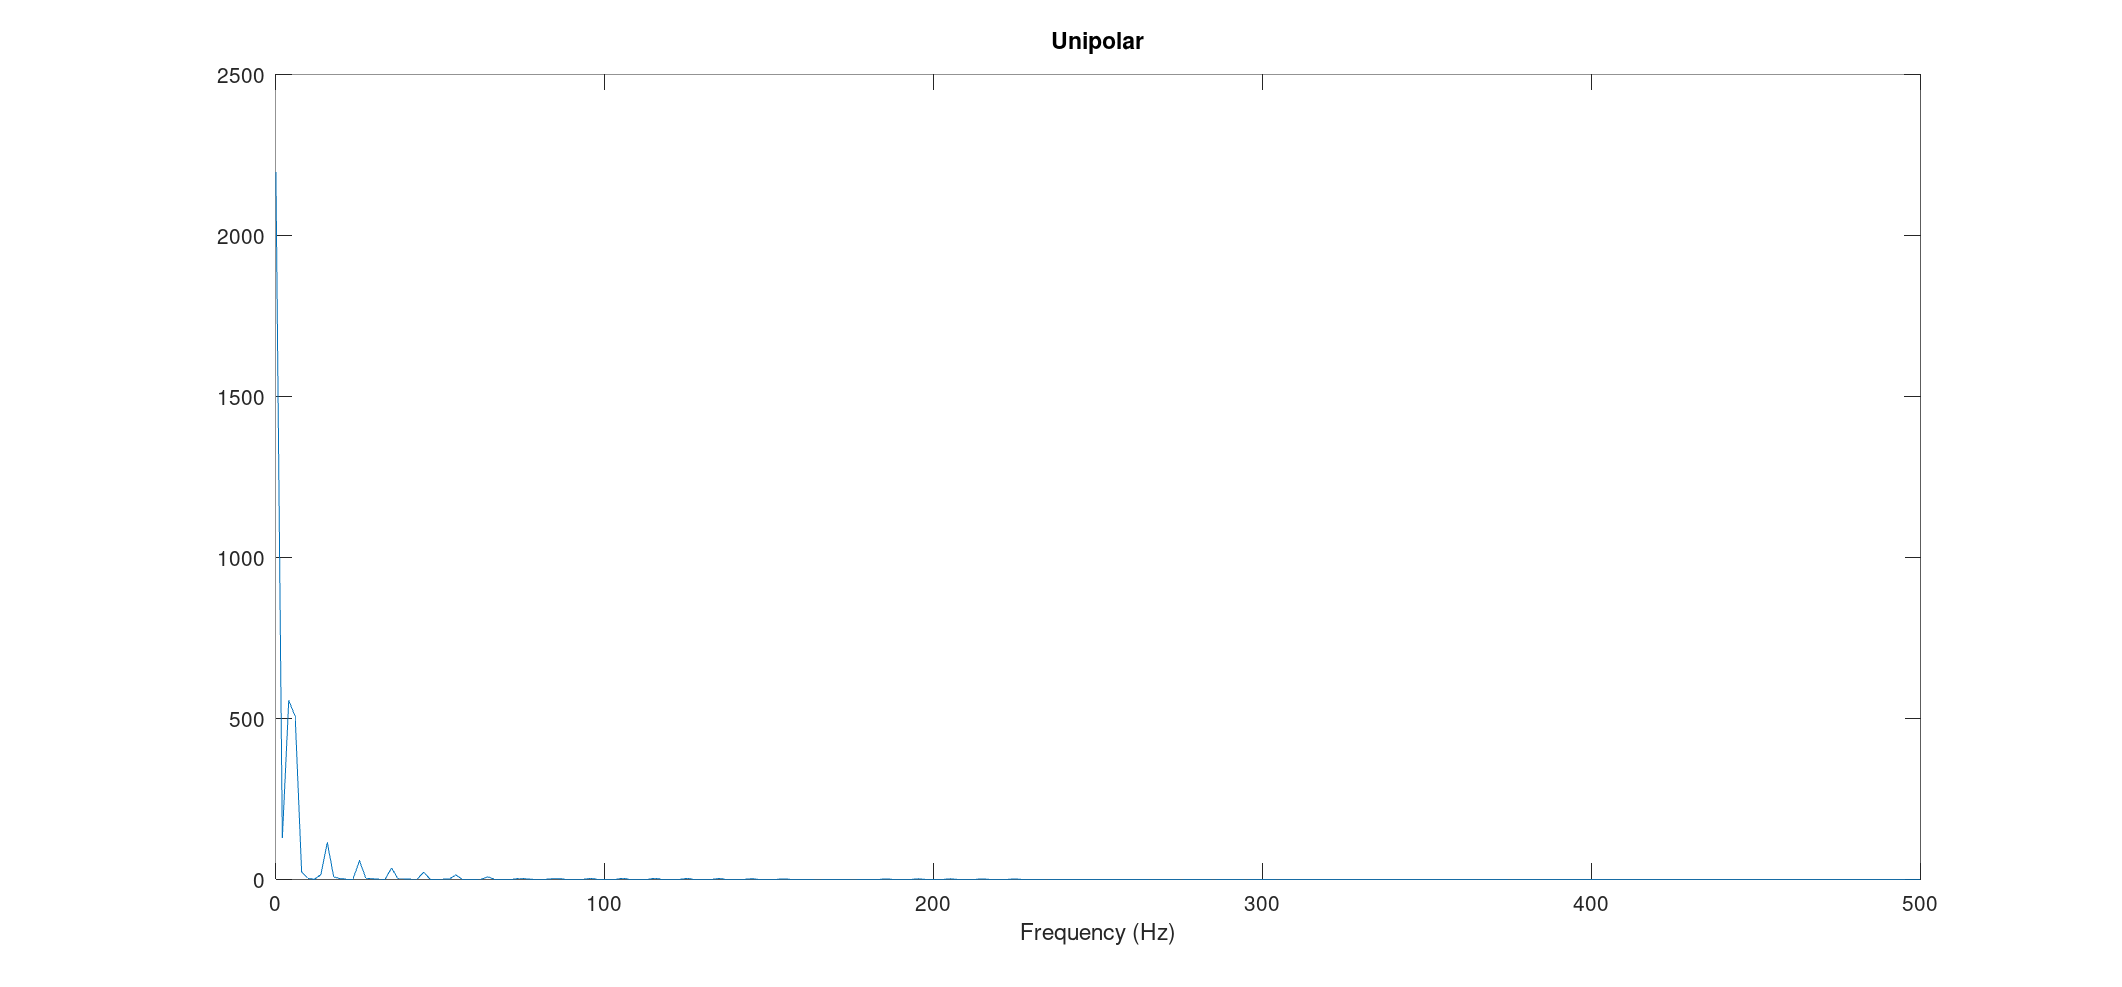
\includegraphics[width=\textwidth]{../octave/coding/spectre/unipolar.png}
            \captionof{figure}{Униполярное кодирование: спектр сигнала}
    \column{0.5\textwidth}
            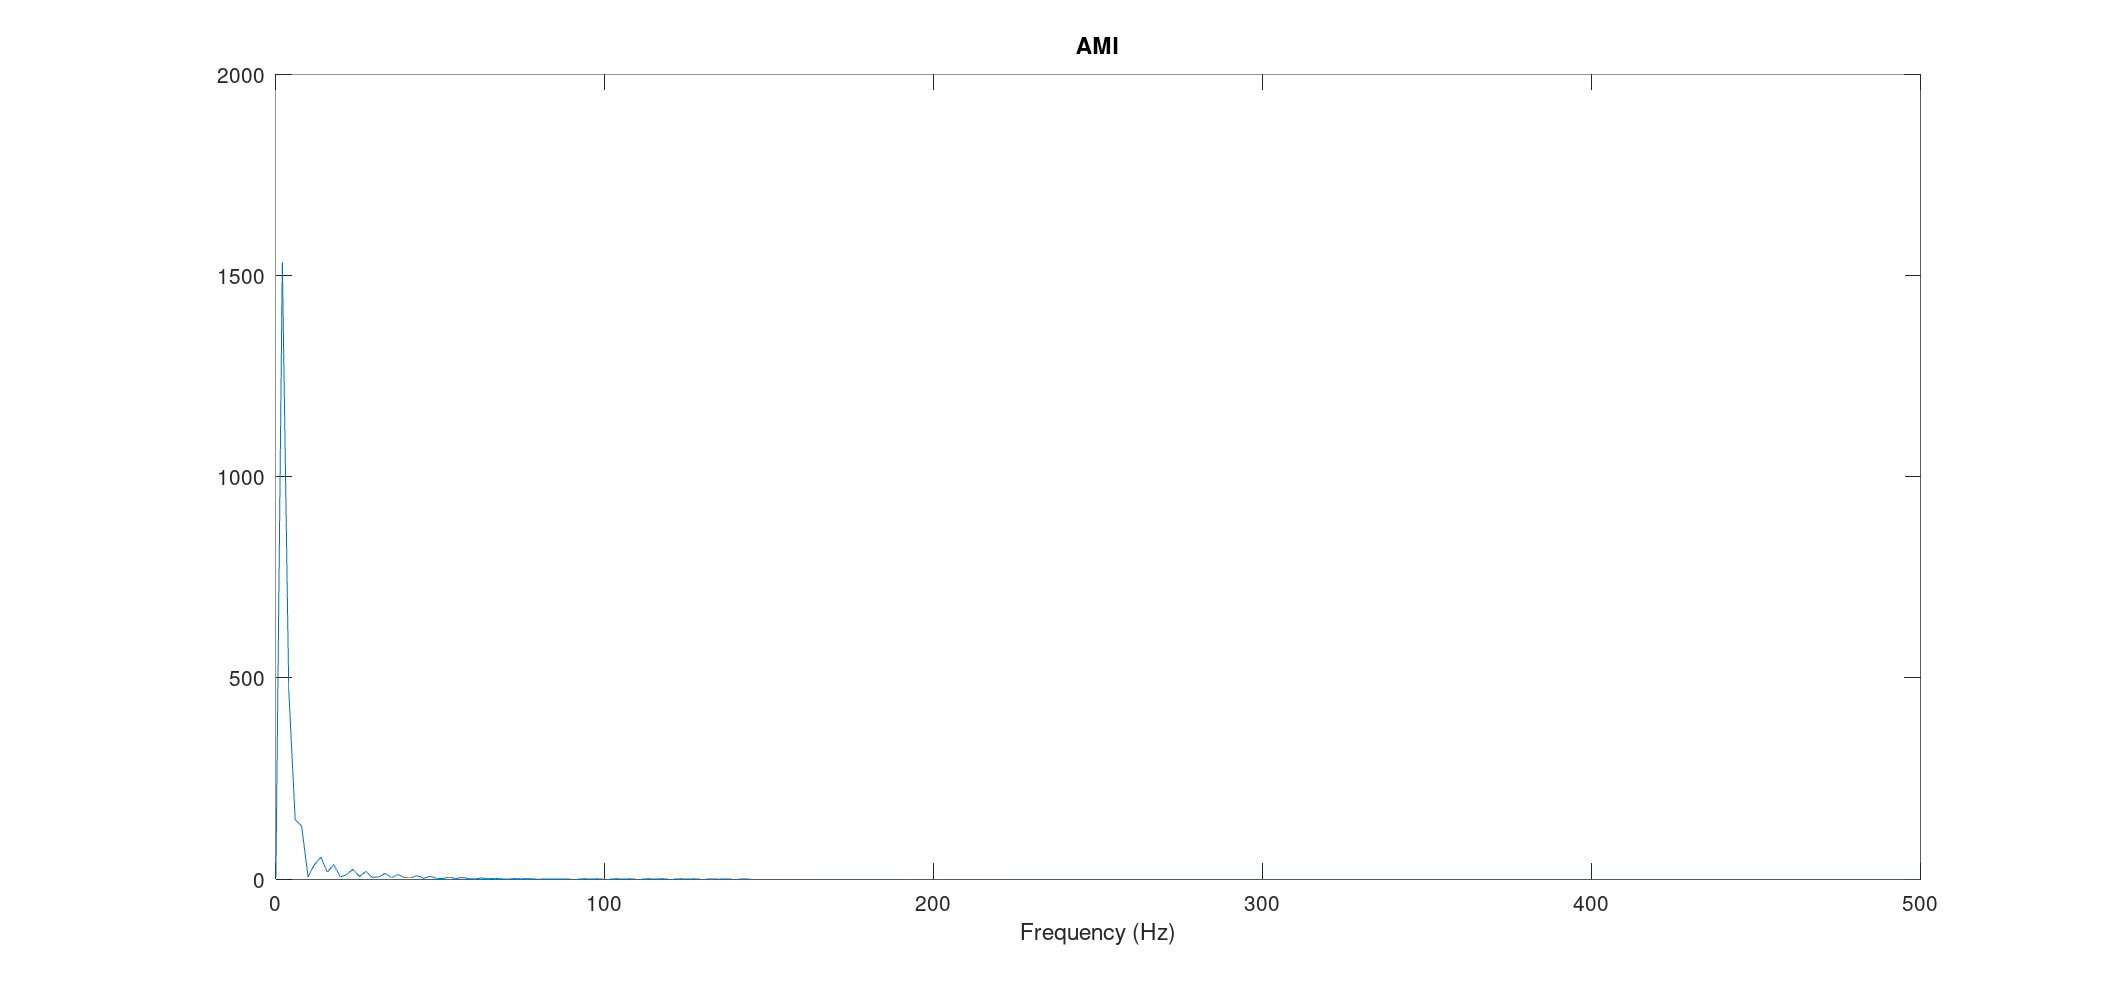
\includegraphics[width=\textwidth]{../octave/coding/spectre/ami.png}
            \captionof{figure}{Кодирование AMI: спектр сигнала}
\end{columns}
\end{frame}

\begin{frame}
\frametitle{Кодирование сигнала. Исследование свойства самосинхронизации сигнала}
\begin{columns}
    \column{0.5\textwidth}
            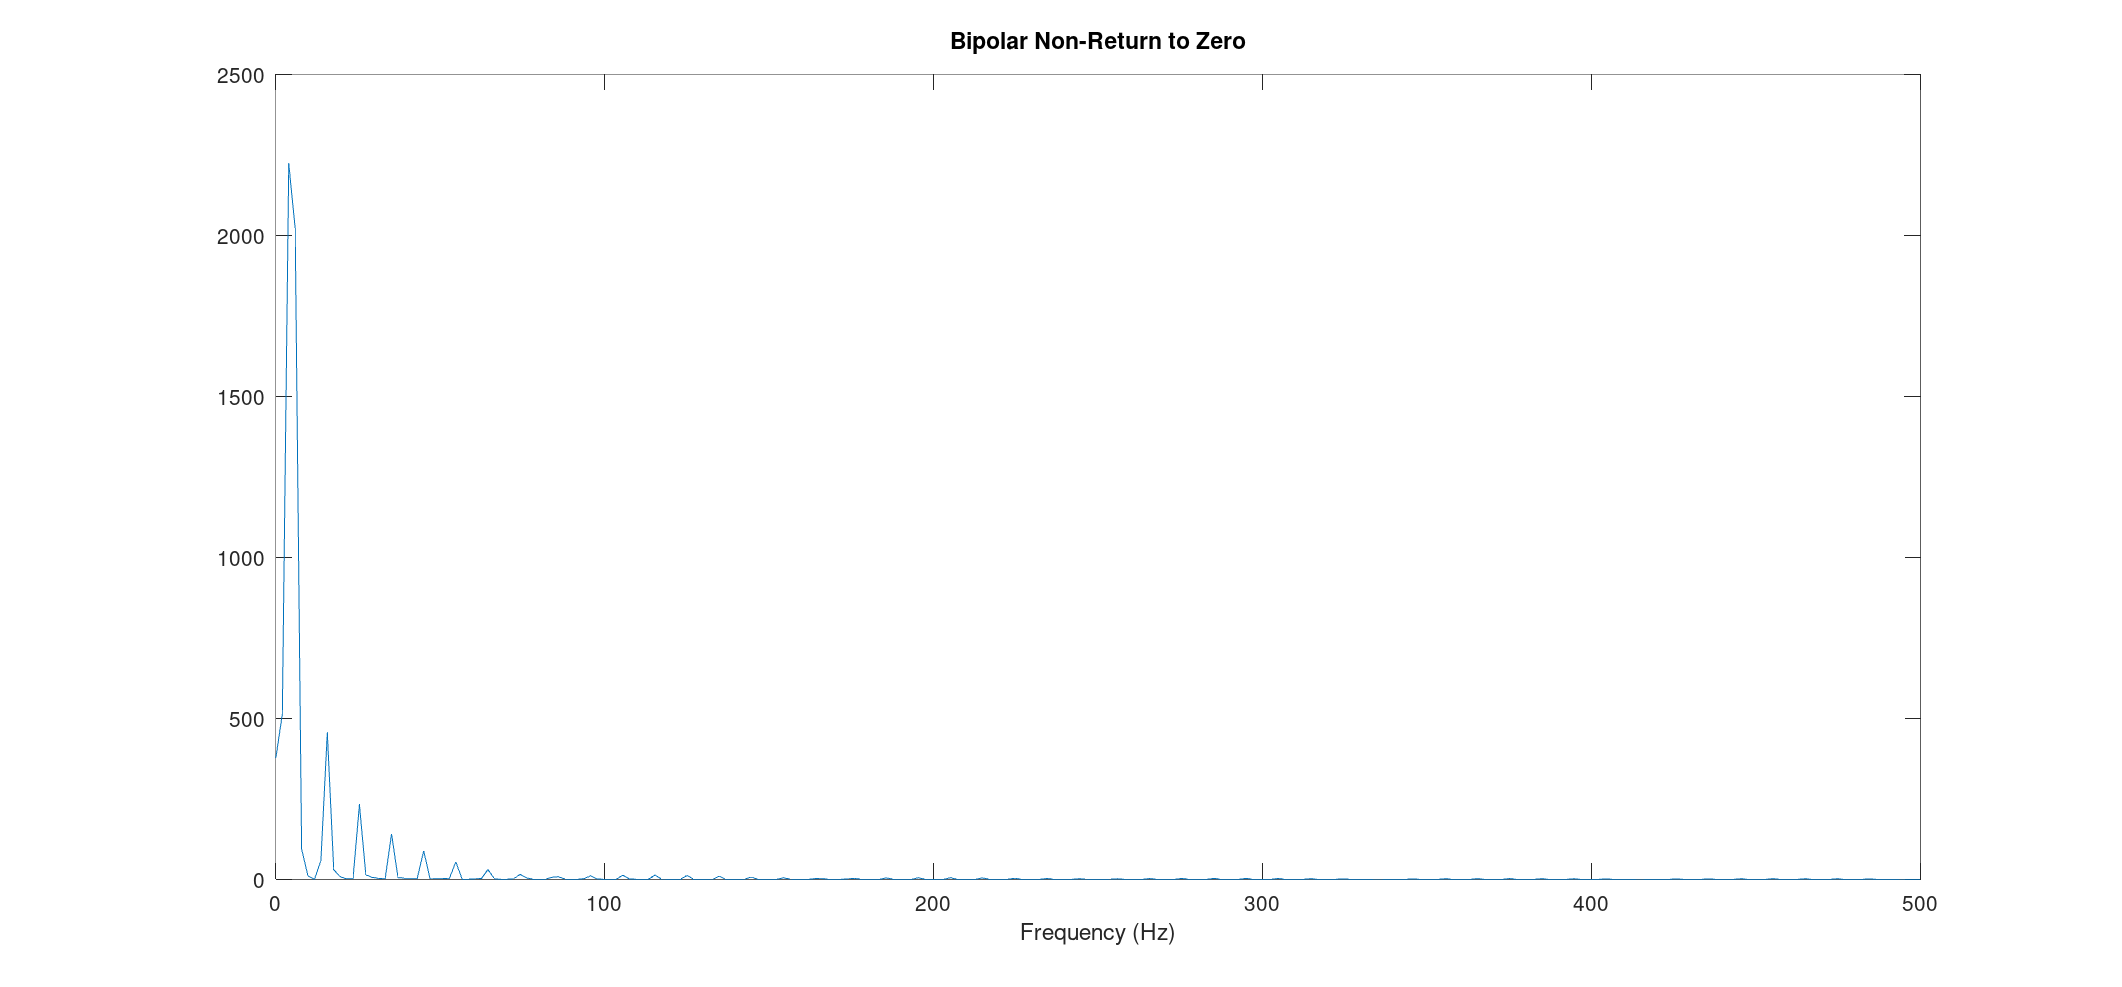
\includegraphics[width=\textwidth]{../octave/coding/spectre/bipolarnrz.png}
            \captionof{figure}{Кодирование NRZ: спектр сигнала}
    \column{0.5\textwidth}
            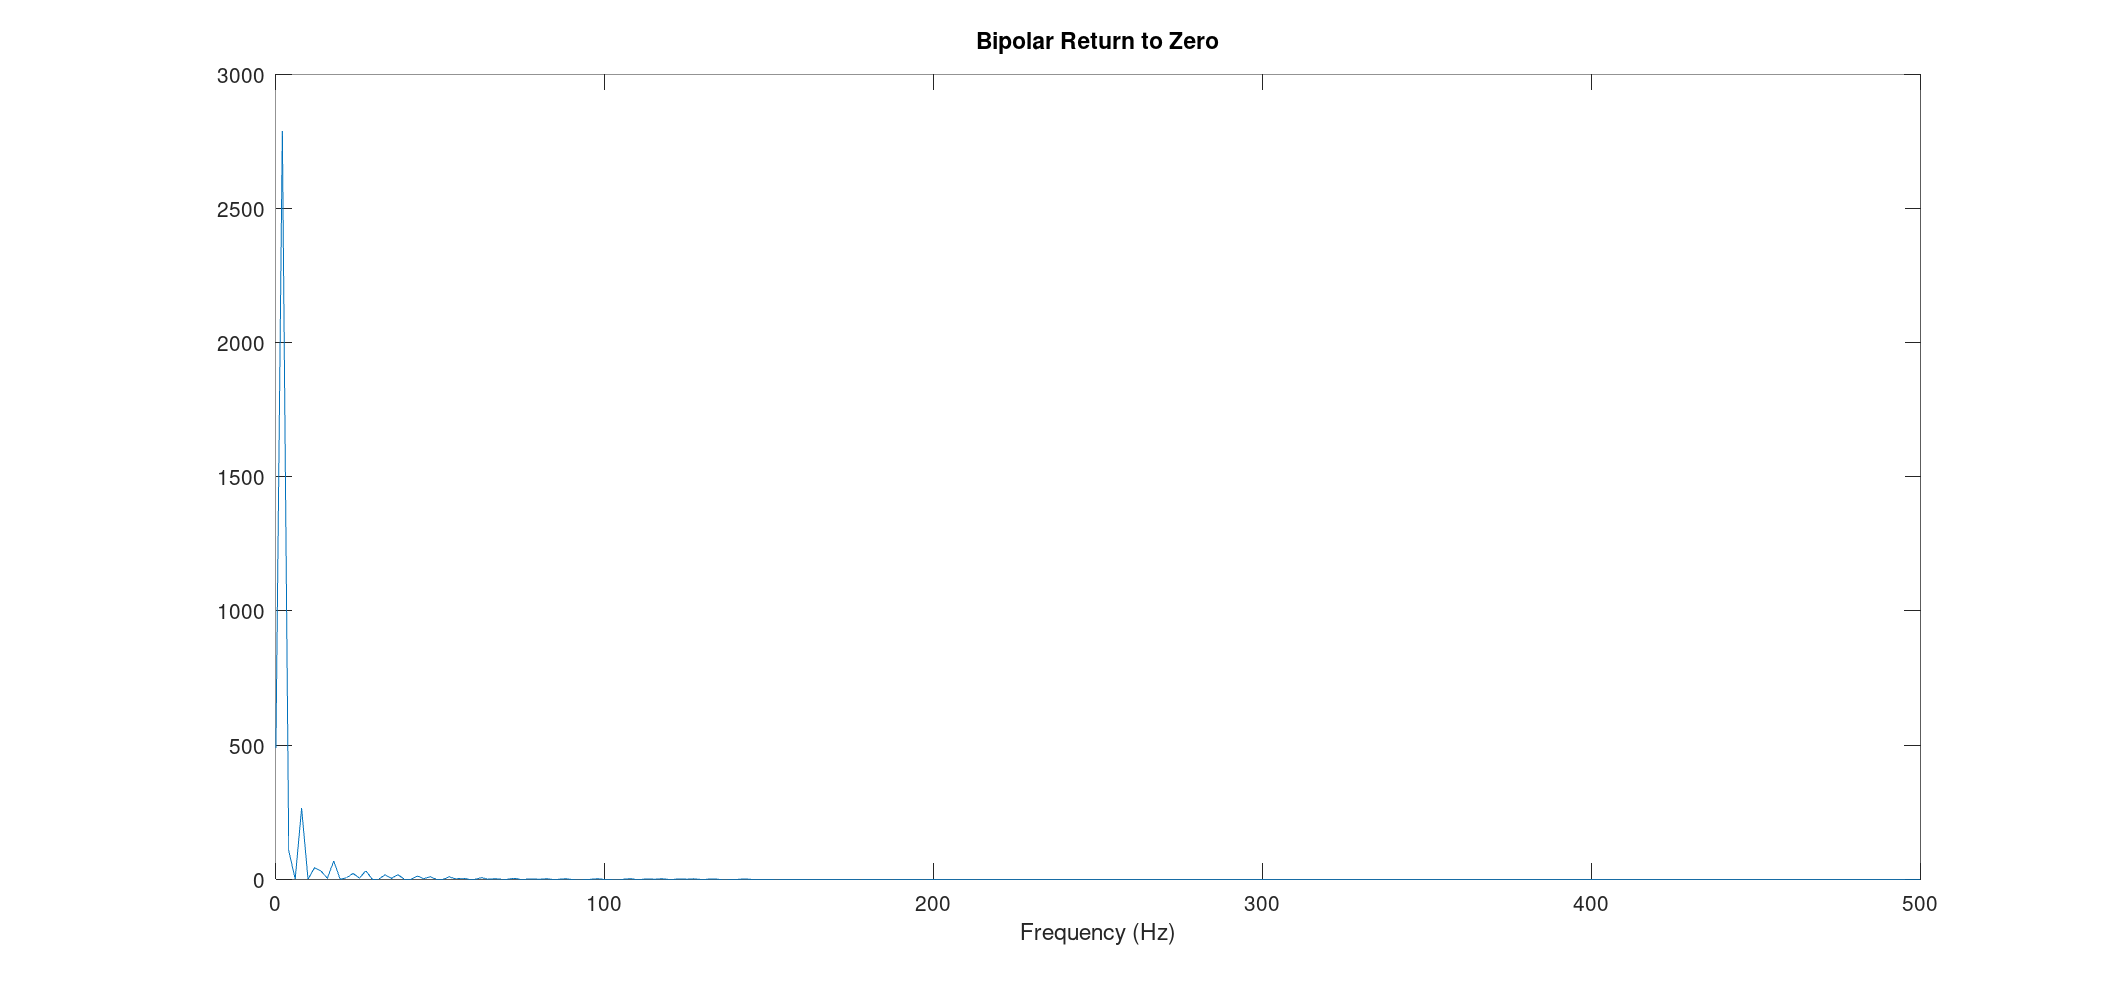
\includegraphics[width=\textwidth]{../octave/coding/spectre/bipolarrz.png}
            \captionof{figure}{Кодирование RZ: спектр сигнала}
\end{columns}
\end{frame}

\begin{frame}
\frametitle{Кодирование сигнала. Исследование свойства самосинхронизации сигнала}
\begin{columns}
    \column{0.5\textwidth}
            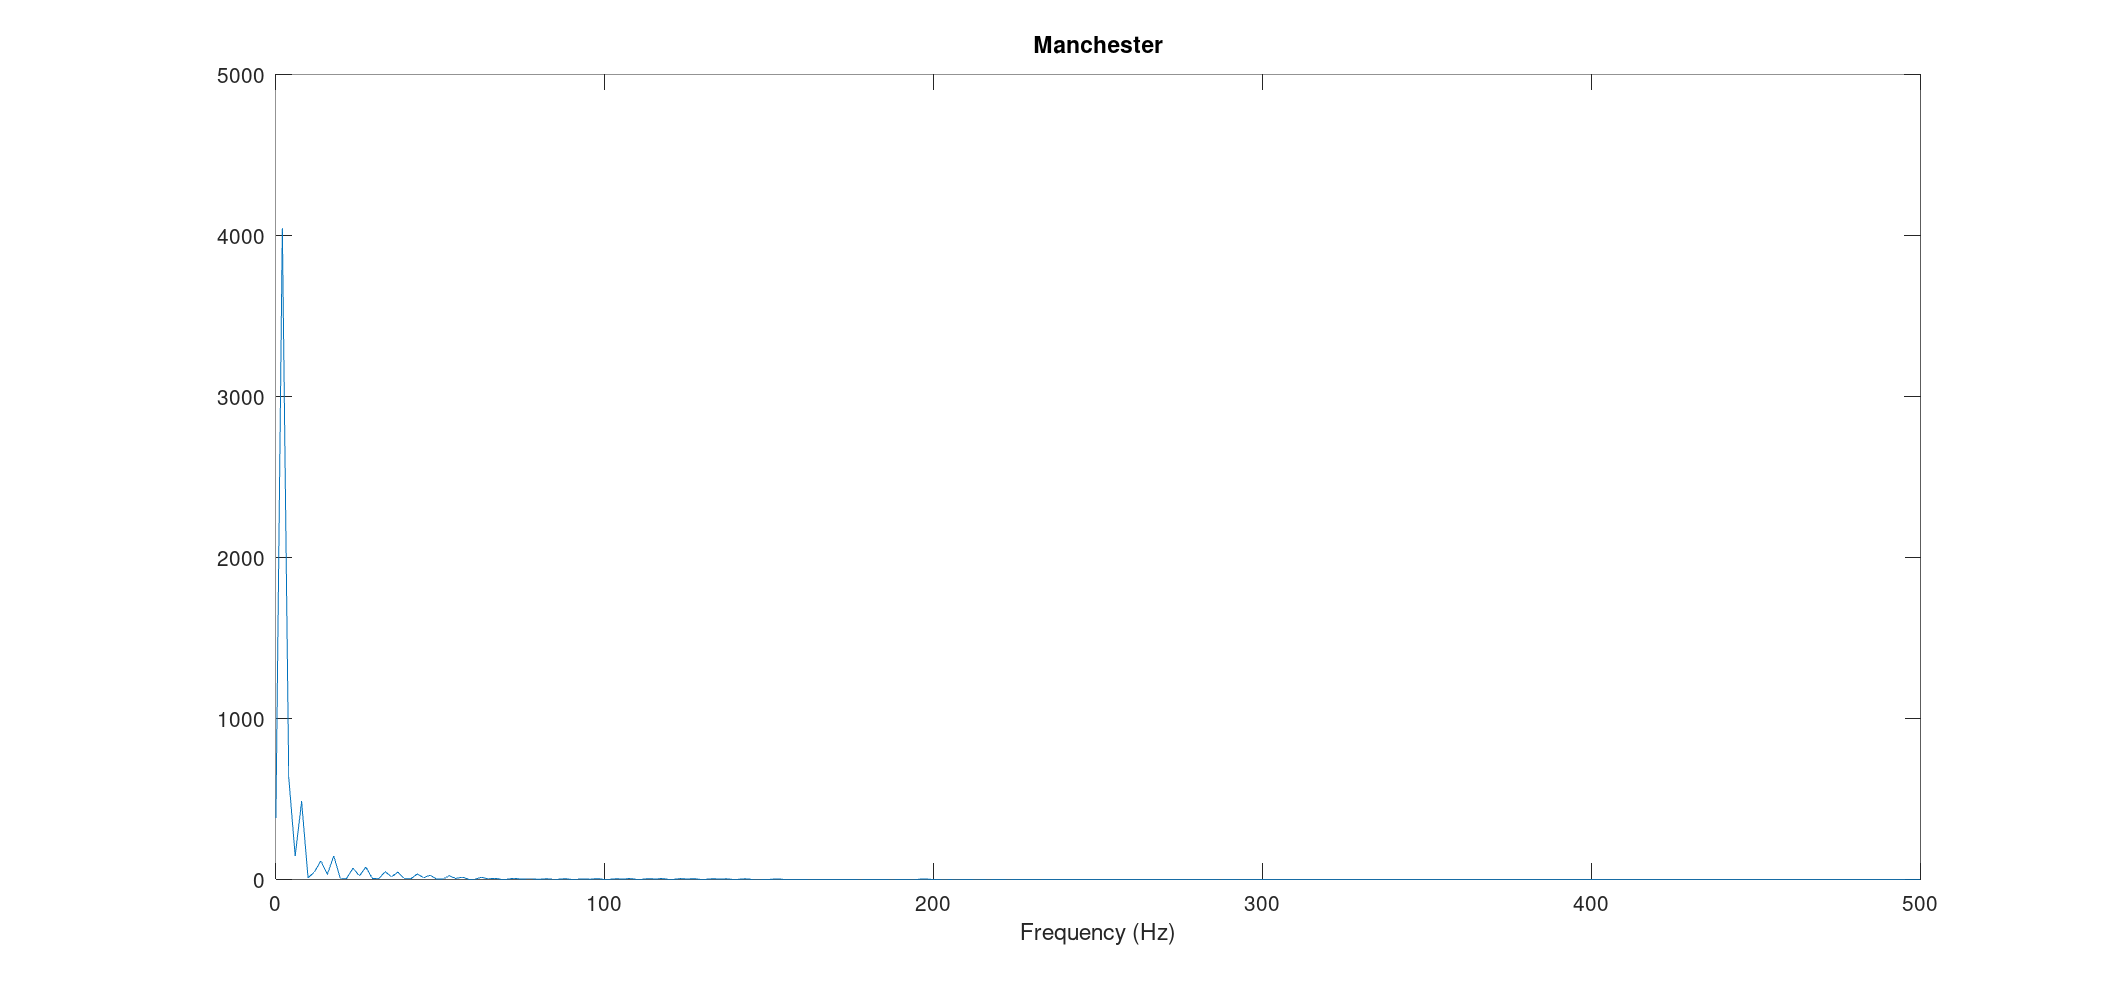
\includegraphics[width=\textwidth]{../octave/coding/spectre/manchester.png}
            \captionof{figure}{Манчестрерское кодирование: спектр сигнала}
    \column{0.5\textwidth}
            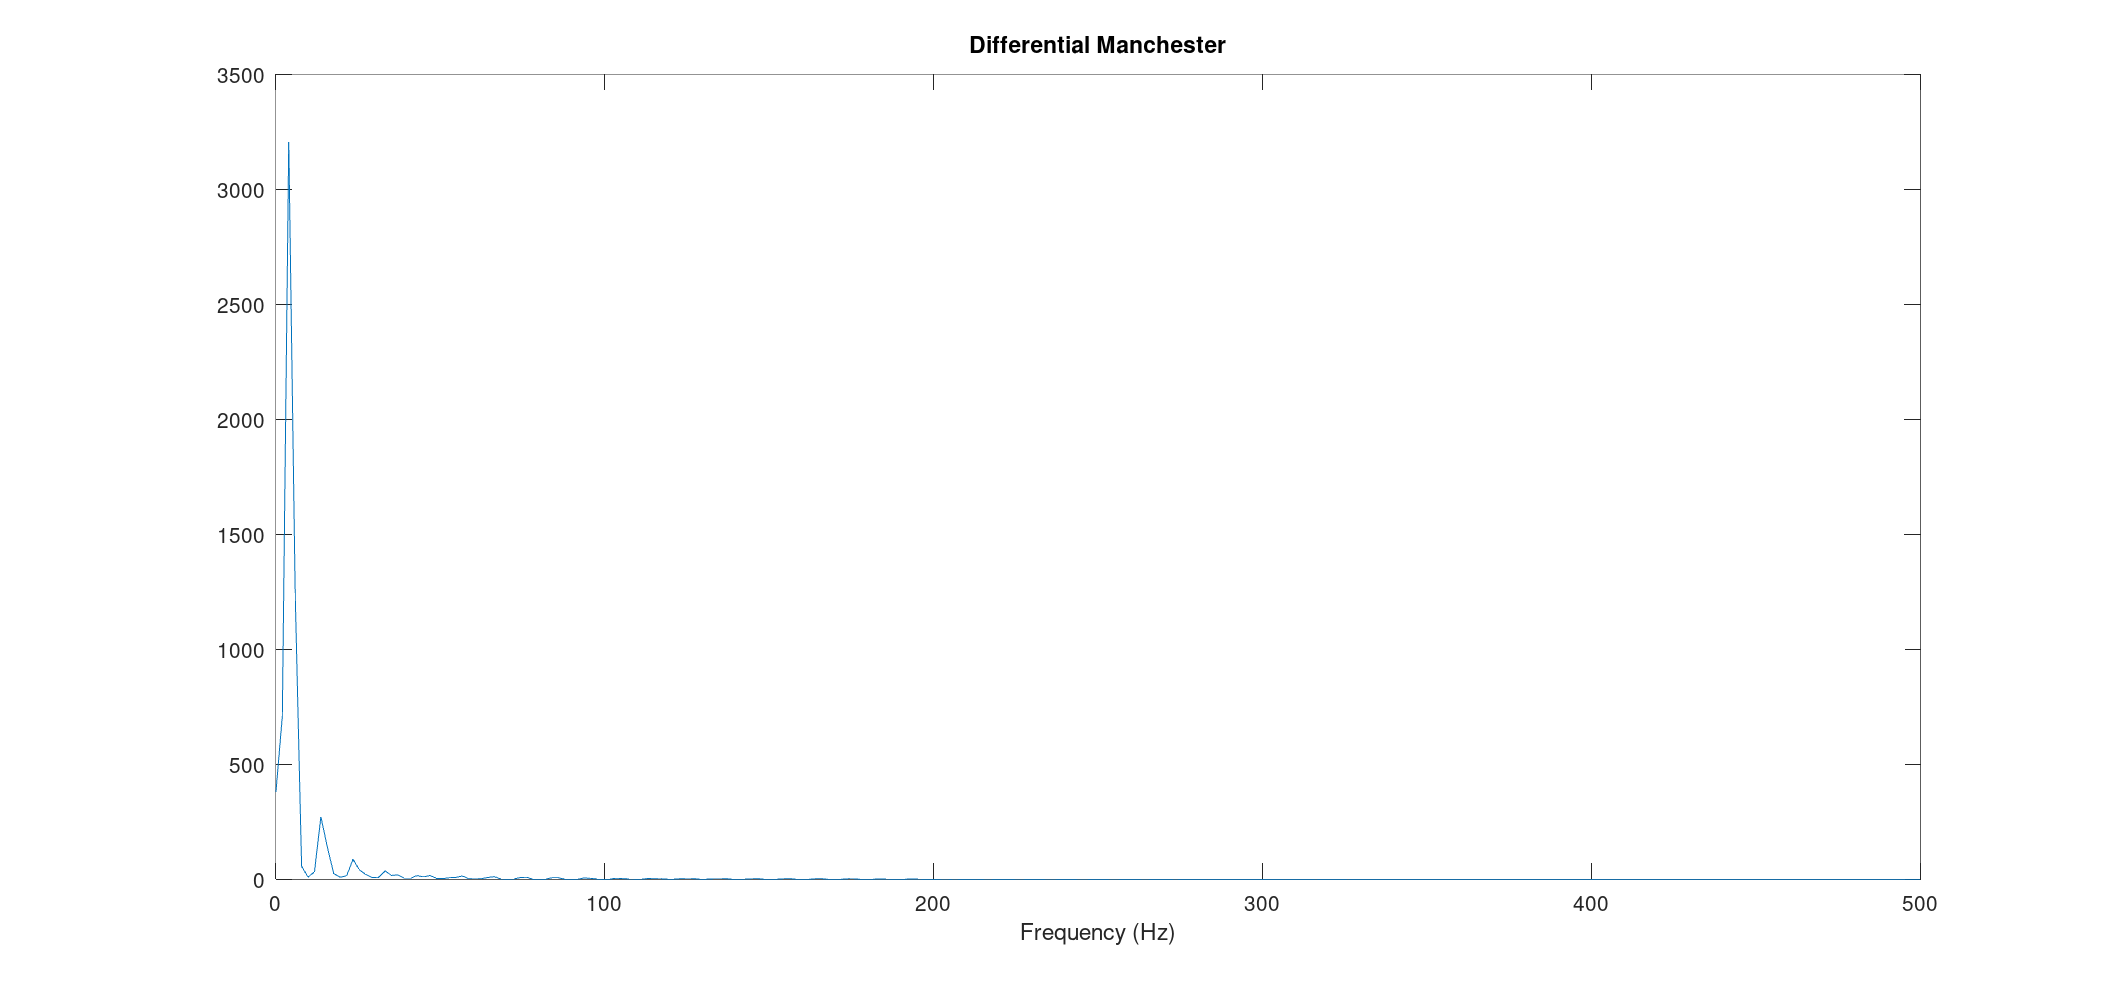
\includegraphics[width=\textwidth]{../octave/coding/spectre/diffmanc.png}
            \captionof{figure}{Дифференциальное манчестерское кодирование: спектр сигнала}
\end{columns}
\end{frame}
\begin{frame}
\frametitle{Выводы}
\begin{itemize}
    \item В рамках выполнения лабораторной работы изучили методы кодирования и модуляции
сигналов с помощью высокоуровнего языка программирования Octave, в том числе
познакомились с принципами модуляции сигнала на примере аналоговй амплитудной
модуляции, исследовали свойства самосинхронизации сигнала.
\end{itemize}
\end{frame}
\end{document}
